\documentclass[conference]{IEEEtran}

\ifCLASSINFOpdf
  % \usepackage[pdftex]{graphicx}
  % declare the path(s) where your graphic files are
  % \graphicspath{{../pdf/}{../jpeg/}}
  % and their extensions so you won't have to specify these with
  % every instance of \includegraphics
  % \DeclareGraphicsExtensions{.pdf,.jpeg,.png}
\else
  % or other class option (dvipsone, dvipdf, if not using dvips). graphicx
  % will default to the driver specified in the system graphics.cfg if no
  % driver is specified.
  % \usepackage[dvips]{graphicx}
  % declare the path(s) where your graphic files are
  % \graphicspath{{../eps/}}
  % and their extensions so you won't have to specify these with
  % every instance of \includegraphics
  % \DeclareGraphicsExtensions{.eps}
\fi

\usepackage[utf8]{inputenc} % allow utf-8 input
\usepackage[T1]{fontenc}    % use 8-bit T1 fonts
\usepackage{url}            % simple URL typesetting

\usepackage{booktabs}       % professional-quality tables
\usepackage{caption}

\usepackage{amsfonts}       % blackboard math symbols
\usepackage{nicefrac}       % compact symbols for 1/2, etc.
\usepackage{microtype}      % microtypography
\usepackage{xcolor}         % colors
\usepackage{graphicx}

% Since ieee redefined proof.
\let\proof\relax \let\endproof\relax
\usepackage{amsthm}

% Copy ieee and use QEDClosed
\renewcommand{\qedsymbol}{$\QEDclosed$}

\usepackage{amsmath}
\usepackage{mathtools}
\usepackage{tabularx}
\usepackage{framed}
\usepackage{bbm}
\usepackage{bm}
\usepackage{xspace}
\usepackage{amssymb}
\usepackage{multirow}
\usepackage{physics}
\usepackage{siunitx}
\usepackage{algorithm}
\usepackage{algorithmic}

% Citation??
\usepackage{cite}

% % Balance references.
% \usepackage{balance}

% Redefined intertext
\usepackage{nccmath}

% Colored cells
\usepackage{colortbl}

% FloatBarrier.
\usepackage{placeins}

\usepackage{subcaption}

\usepackage{lipsum}

% % Proofs at the end because ICRA double column is super hard to write proofs with.
% \usepackage[createShortEnv,conf={end,restate,no link to proof}]{proof-at-the-end}
\usepackage{thmtools}
\usepackage{thm-restate}

% % Proof Sketches
% \usepackage{apxproof}

% \declaretheorem{lemma}

% % Show the label for equations.
% \providecommand*\showkeyslabelformat[1]{%
% \setlength{\fboxsep}{1pt}
% \fbox{\normalfont\fontsize{4.5}{5.4}\ttfamily#1}}
% \usepackage[notref,notcite]{showkeys}

% Allow hyperlinks to work.
\makeatletter
\let\NAT@parse\undefined
\makeatother
\usepackage{hyperref}       % hyperlinks
\hypersetup{
    colorlinks,
    linkcolor={blue!90!black},
    citecolor={blue!90!black},
    % citecolor={green!80!black},
    urlcolor={blue!95!black}
}

\usepackage[capitalise]{cleveref}       % Named refs
\usepackage{crossreftools}  % Fix cleveref in headers.
\pdfstringdefDisableCommands{%
    \let\cref\crtcref
    \let\cref\crtcref
}

\usepackage[all=normal,paragraphs=tight,floats=tight,mathspacing=tight,wordspacing=tight,tracking=tight]{savetrees}
\newcommand*\numx{n_{\vx}}
\newcommand*\numu{n_{\vu}}


\newcommand*\negi{{\neg i}}

\newcommand*\ui{u^{i}}
\newcommand*\unegi{{\vu}^{\negi}}
\newcommand*\Unegi{{\vU}^{\negi}}

\newcommand*\pii{\pi^{i}}
\newcommand*\piis{{\pi}^{i*}}
\newcommand*\pinegi{\vpi^{\negi}}
\newcommand*\pinegis{{\vpi}^{\negi*}}

\newcommand*\vdx{\delta \vx}
\newcommand*\vdu{\delta \vu}
\newcommand*\vdus{{\delta \vu^*}}
\newcommand*\vdunegi{\delta {\vu^{\negi}}}
\newcommand*\vdunegis{\delta {\vu^{\negi*}}}

\newcommand*\deluis{\delta {u^{i*}}}
\newcommand*\delu{\delta u}
\newcommand*\delui{\delta {u^i}}
\newcommand*\ddelui{\dif \delta {u^i}}
\newcommand*\tildedelui{{\delta {\tilde{u}^i}}}

% \newcommand{\one}{{(\mathfrak{1})}}
% \newcommand{\two}{{(\mathfrak{2})}}
\newcommand{\one}{{\mathfrak{1}}}
\newcommand{\two}{{\mathfrak{2}}}

\newcommand{\notone}{{\neg \mathfrak{1}}}

%%%%%%%%%%%%%%%%%%%%%%%%%%%%%
%        POMDP
%%%%%%%%%%%%%%%%%%%%%%%%%%%%%
\newcommand*\QMDP{\textrm{QMDP}}
\newcommand*\FIB{\textrm{FIB}}

%%%%%%%%%%%%%%%%%%%%%%%%%%%%%
%        Methods
%%%%%%%%%%%%%%%%%%%%%%%%%%%%%
\newcommand*\ttNoInf{{\texttt{NoInf}}}
\newcommand*\ttYield{{\texttt{Yield}}}
\newcommand*\ttNoYield{{\texttt{NoYield}}}
\newcommand*\ttML{{\texttt{ML}}}
% \newcommand*\ttQMDP{{\texttt{QMDP}}}
\newcommand*\ttQMDP{{\texttt{MPOGames}}}

\newtheorem{lemma}{Lemma}
\newtheorem*{remark}{Remark}

\newenvironment{proofsketch}{\begin{proof}[Proof sketch]}{\end{proof}}

%%%%%%%%%%%%%%%%%%%%%%%%%%%%%
%        DOMAINS
%%%%%%%%%%%%%%%%%%%%%%%%%%%%%
\newcommand*{\Rb}{\mathbb{R}}

%%%%%%%%%%%%%%%%%%%%%%%%%%%%%
%        Math Operators
%%%%%%%%%%%%%%%%%%%%%%%%%%%%%
\DeclareMathOperator*{\Eb}{\mathbb{E}}


% \DeclareMathOperator*{\SM}{\textrm{SM}}
\DeclareMathOperator*{\SM}{\sigma_{\textrm{SM}}}

\DeclareMathOperator*{\argmin}{\arg\!\min}
\DeclareMathOperator*{\argmax}{\arg\!\max}

%%%%%%%%%%%%%%%%%%%%%%%%%%%%%
%        OTHER
%%%%%%%%%%%%%%%%%%%%%%%%%%%%%
\newcommand{\T}{^\mathsf{T}}
\DeclareMathOperator*{\ego}{ego}
\newcommand{\todo}[1]{\textcolor{red}{[todo: #1]}}
\newcommand{\softmax}{\textnormal{softmax}}
\newcommand{\bl}[1]{{\color{blue} #1}}

%%%%%%%%%%%%%%%%%%%%%%%%%%%%%
%        BOLD SYMBOLS
%%%%%%%%%%%%%%%%%%%%%%%%%%%%%
\def\vk{{\vb{k}}}
\def\vu{{\vb{u}}}
\def\vx{{\vb{x}}}

\DeclareBoldMathCommand\vpi{\pi}

\def\vK{{\vb{K}}}
\def\vU{{\vb{U}}}
\def\vX{{\vb{X}}}


% correct bad hyphenation here
\hyphenation{op-tical net-works semi-conduc-tor tele-opera-tion bi-manual}


\begin{document}
%
% paper title
% Titles are generally capitalized except for words such as a, an, and, as,
% at, but, by, for, in, nor, of, on, or, the, to and up, which are usually
% not capitalized unless they are the first or last word of the title.
% Linebreaks \\ can be used within to get better formatting as desired.
% Do not put math or special symbols in the title.
\title{Vision-Mediated Decentralized Coordination \\
for Bimanual Tray Lifting with \\
SO-101 Arms}


% author names and affiliations
% use a multiple column layout for up to three different
% affiliations
\author{\IEEEauthorblockN{Jackson Crocker}
\IEEEauthorblockA{Mechanical and Aerospace Engineering\\
Princeton University\\
Princeton, NJ, USA\\
jackson.crocker@princeton.edu}
\and
\IEEEauthorblockN{David Herrera}
\IEEEauthorblockA{Mechanical and Aerospace Engineering\\
Princeton University\\
Princeton, NJ, USA\\
davidherrera@princeton.edu}}




% make the title area
\maketitle
% As a general rule, do not put math, special symbols or citations
% in the abstract
\begin{abstract}
We present a decentralized algorithmic approach to bimanual tray-lifting with two independent LeRobot SO-101 robot arm manipulators. The two arms share only a single RGB camera stream and exchange no direct messages of any kind. Each arm runs in its own thread and issues motor commands from a scene representation it builds for itself from AprilTag markers on the tray, grippers, and arm bases. Coordination emerges implicitly from both arms observing the same scene and mapping observations to joint commands through the same pipeline. This pipeline includes a pre-fit polynomial motion map from base-frame planar coordinates to joint angles, a shared phased procedure, and closed-loop visual servoing. The contribution of this paper is a set of coordination primitives for bimanual lifting that rely only on shared vision:
(i) a \emph{nudge-lift handshake} in which each arm pre-tensions the tray and waits for a rise on the opposing tray marker before commencing the full lift; (ii) a \emph{tilt-aware synchronized lift} in which each arm throttles its own ascent based on the relative height of the two tray markers; 
(iii) a \emph{leader--follower translation} in which the follower tracks the leader's gripper marker through a once-measured offset; and 
(iv) a \emph{tilt-aware lower} that pauses the lower side of the tray so the other side catches up. The full sequence executes reliably on physical hardware with a water-filled glass on the tray, demonstrating that
non-trivial bimanual manipulation can be achieved without an explicit communication channel.
\end{abstract}

\begin{figure}[h]
    \centering
    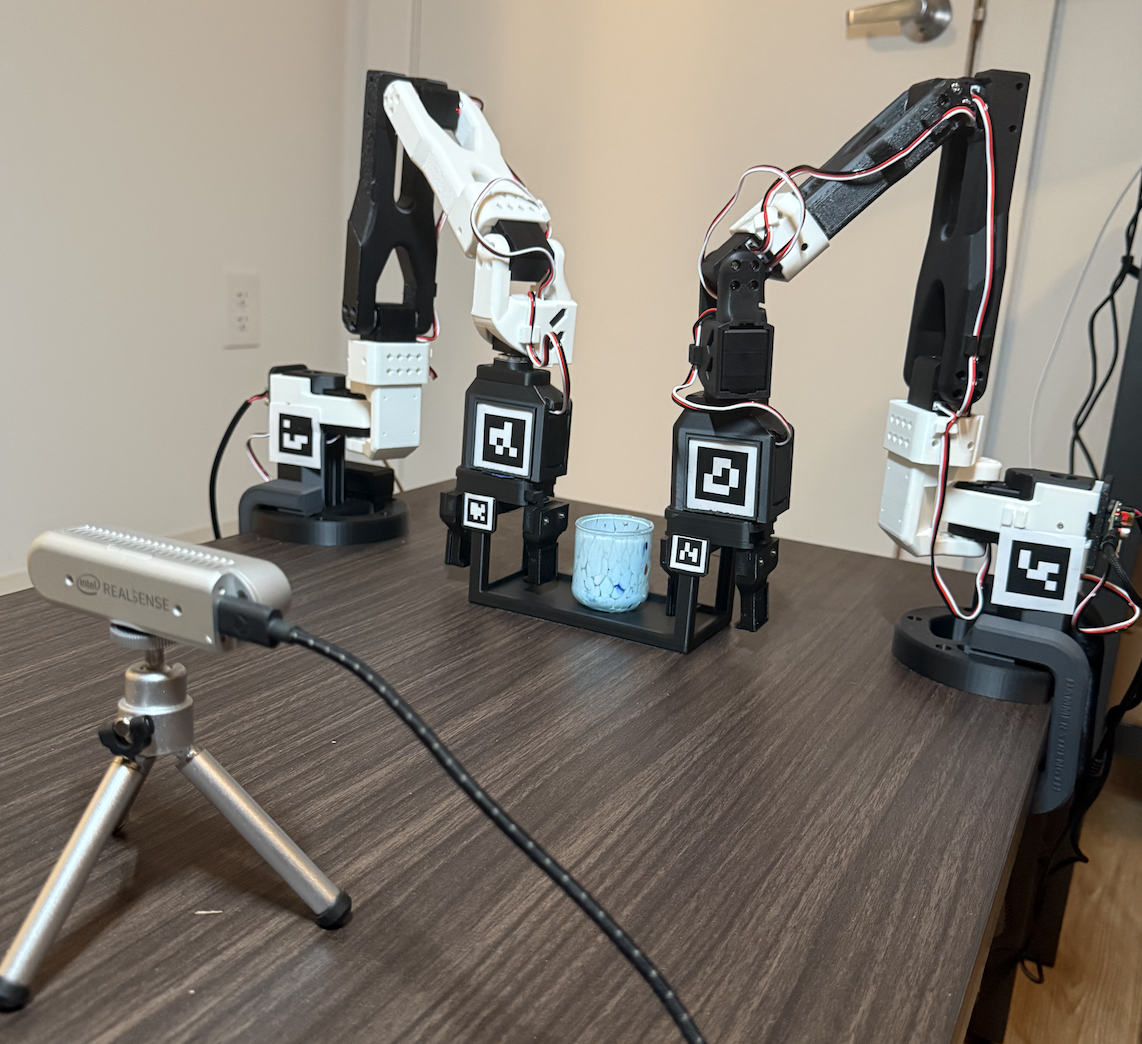
\includegraphics[width=1\linewidth]{subtex/images/main_image.png}
    \caption{Problem Setup}
    \label{fig:Project Setup}
\end{figure}


% For peer review papers, you can put extra information on the cover
% page as needed:
% \ifCLASSOPTIONpeerreview
% \begin{center} \bfseries EDICS Category: 3-BBND \end{center}
% \fi
%
% For peerreview papers, this IEEEtran command inserts a page break and
% creates the second title. It will be ignored for other modes.
\IEEEpeerreviewmaketitle

\section{Introduction}

Bimanual manipulation of large or awkward objects is a classic challenge in robotics: the two end-effectors are kinematically independent, but the object they jointly hold couples their behavior. Mistimed or mismatched motion immediately produces forces, tilts, or slips that ruin the task. In practice this is almost always solved by explicit coordination which includes a central planner, a shared controller, or a communication channel that exchanges orientation, forces, or high-level intent~\cite{smith2012dualarm}.

This paper asks a more restrictive question. Suppose we forbid the two arms from talking to each other at all. Each arm runs as an independent process with its own controller, its own sense of time, and its own view of the world through a shared RGB camera. Can two arms, given only what they see, coordinate tightly enough to lift a tray with a glass of water on it, move it across the table, and set it down without spilling? This is a robotics realization of tacit coordination where independent agents converge on aligned behavior through shared context rather than explicit messaging.

We show that the answer is yes, and that the coordination required is not hidden inside a machine learning black box. It can be written as a handful of small, interpretable algorithms whose only shared state is the image and the object identities. The two arms run identical software and coordination emerges because both arms look at the same markers and respond to them with the same deterministic pipeline.

\subsection{Problem Setup}
Two LeRobot SO-101 5-DoF follower arms are mounted facing each other on a table, separated by roughly 40 centimeters, as seen in Figure \ref{fig:Project Setup}. A single Intel RealSense D435i camera provides a 640$\times$480 RGB stream (depth is not used). Six fiducial (tag16h5) markers are placed in the scene: one on each arm base, one on each gripper, and two on opposite sides of the tray. A glass is placed near the tray center and spill risk is simply encoded by the height difference between the two tray markers.
The system must execute a complete pick-move-place: approach the tray, grasp it from both sides, lift it level, translate it backward, lower it, and release.

\subsection{Contributions}
The contributions of this paper are algorithmic and focused on the coordination problem. Specifically, we contribute:
\begin{itemize}
\item A \textbf{motion-map formulation} that decouples perception from control: each arm uses a polynomial
$(x,z) \!\to\! \text{joint angles}$ fit from a manually-collected workspace sweep, so runtime servoing is a polynomial evaluation plus a feedback correction rather than an inverse-kinematics solve. This system allows for limited empirical inverse kinematics on arbitrary (and under-actuated) hardware.
\item A \textbf{finite-state coordination protocol}
(\cref{sec:coordination}) in which both arms run the same
state machine and transitions are triggered by visual events rather than messages.
\item A \textbf{nudge-lift handshake} that replaces any explicit
ready-to-lift messaging with a small physical pre-move on the tray, detected by the opposite arm as a vertical rise on the tray marker.
\item A \textbf{tilt-aware synchronized lift} rule that keeps the tray within a few millimeters of level during ascent by having each arm throttle its own motion based on the relative height of the two tray markers.
\item A \textbf{leader--follower translation} that uses the leader's gripper marker with a once-measured offset mapping leader gripper to follower tray target.
\end{itemize}

\subsection{Paper Organization}
\cref{sec:related} briefly positions the work in other bimanual
manipulation literature. \cref{sec:system} describes the hardware and software systems. \cref{sec:perception} covers the perception pipeline and the base-frame calibration that makes control generalizable to other environments. \cref{sec:motionmap} explains the polynomial motion map. \cref{sec:coordination} is the core of the paper: it presents the full phasing protocol and coordination algorithms with pseudocode. \cref{sec:results} reports hardware trials, and \cref{sec:conclusion} concludes.

\section{Related Work}
\label{sec:related}

\subsection{Bimanual Manipulation}
Bimanual manipulation has a long history in both classical control and, more recently, machine learning. The literature review of Smith \emph{et al.}~\cite{smith2012dualarm} organizes the two arm literature along two axes: coordination structure (leader-follower, symmetric, or asymmetric) and coupling representation (kinematic constraints, hybrid position/force, or trajectory parameterization). The vast majority of these systems achieve coordination through a shared state vector or a centralized controller. On the learning side, ALOHA / ACT~\cite{zhao2023aloha} showed that a single policy with full access to both arms' states and a shared visual feed can imitate bimanual tasks from a small dataset. Both lines of work share the assumption that ours deliberately violates: that the two arms have access to a common state, controller, or model. We treat the two arms as fully independent processes connected only by what the camera can see.

\subsection{Cooperative Manipulation Without Communication}
Our closest ancestor is the work of Wang and Schwager~\cite{wang2016forceants} on the Force-Amplifying N-Robot Transport System (Force-ANTS). They demonstrate that a team of mobile robots can cooperatively transport a heavy object without communication, by having each robot independently estimate the object's velocity and apply forces in the same direction. Our system differs in three areas: the shared signal is visual rather than force-based; the object geometry is exploited explicitly (the tray's two markers estimate tilt); and the task progresses through discrete coordination events, rather than a single continuous transport. The underlying principle, however, is the same in that each agent computes something locally from a signal that captures the team's joint state.

\subsection{Visual Servoing and Marker-Based Perception}
The runtime control loop is a position-based visual servo (PBVS)~\cite{chaumette2006visual1}: at each tick we measure the pose error of the gripper relative to a tray marker in the Cartesian frame and command the joints to reduce that error. We rely on fiducial markers~\cite{garrido2014aruco} for pose extraction, using OpenCV's ArUco module configured with the AprilTag 16h5 library~\cite{olson2011apriltag} for their easy to make and large codes. At our 0.3-0.8 m visual operating range, the per-marker pose estimate from \texttt{cv2.solvePnP} with \texttt{SOLVEPNP\_IPPE\_SQUARE} produces 5-10 mm 3D accuracy, which is better than the coordination thresholds the algorithms of \cref{sec:coordination} require.

\subsection{Open Hardware and Software Stacks}
We build on the LeRobot framework~\cite{cadene2026lerobot} for SO-101 motor control, calibration, and bus management. LeRobot provides a uniform Python interface across follower-arm hardware, which lets us treat each arm thread identically up to the port and calibration files. The two SO-101 arms are inexpensive, open-source designs, which makes modifying the hardware and getting started with the software much more accessible.
\section{System Overview}
\label{sec:system}

The system utilizes two identical 5-DoF SO-101 follower arms with a binary end-effector, each with position-controlled Feetech STS3215 servos exposed through HuggingFace LeRobot's~\cite{cadene2026lerobot} \texttt{SOFollower} bus interface. A single Intel RealSense D435i camera to one side of the arms provides a 640$\times$480 RGB stream at 30\,fps; only the color stream is used. 


\subsection{AprilTags \& Camera}

Six ArUco markers~\cite{garrido2014aruco} drawn from the AprilTag Tag16h5 dictionary~\cite{olson2011apriltag} label the scene:

\begin{itemize}
  \item Two 40 mm markers, one on each arm base, used for camera-to-base calibration
  \item Two 40 mm markers on the gripper fingers for runtime visual servoing
  \item Two 20 mm markers on opposite sides of the tray, separated by a known horizontal spacing (140 mm), which double as position references and as a tilt gauge via their relative height
\end{itemize}

Understanding the nomenclature of ArUco markers is important to select the appropriate markers for each task. AprilTags are categorized into groups, or "families" depending on their complexity and resistance to error as shown in Figure \ref{fig:apriltag picture}. Within "Tag16h5", the "16" refers to the number of pixels in the tag, in this case a 4 x 4 tag. The "h5" refers to the tag's resistance to error, or how many pixels would need to be perceived incorrectly before the tag is mistaken for a different tag. 

\begin{figure} [H]
    \centering
    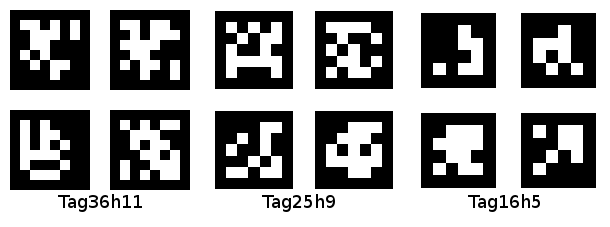
\includegraphics[width=1\linewidth]{subtex//images/AprilTags.png}
    \caption{Three different commonly used AprilTag families}
    \label{fig:apriltag picture}
\end{figure}

Generally, AprilTag families with less detail are used for applications at longer distances. Having less detail allows the tag to be easily discernible and therefore more reliable. Tags such as Tag36h11 contain more pixels as a 6 x 6 grid, and therefore have a higher resistance to error at h11. These tags are used for shorter ranges because they contain more detail and would be harder to percieve at long distances. 

Due to our size constraints, the simpler Tag16h5 AprilTags were used. The relative small scale of our setup simulates a long distance environment. Because our marker sizes were 20 mm for the tray and 40 mm for the end-effectors and we only needed 6 tags total, it was important for the tags to be as simple as possible so they could be read accurately.

These AprilTags were detected by a RealSense D435i Camera shown in Figure \ref{fig:camera}. Although the RealSense camera is capable of infrared (IR) stereo depth perception, it was not used due to noise and unreliability. Instead, steady RGB footage at 30 Hz was utilized. Both robot arms shared context through this camera, but because they run in separate threads, this simulates having two cameras placed in the same position. Two cameras would have been preferred for added generalizability, but resource constraints prohibited this augmentation.

\begin{figure} [H]
    \centering
    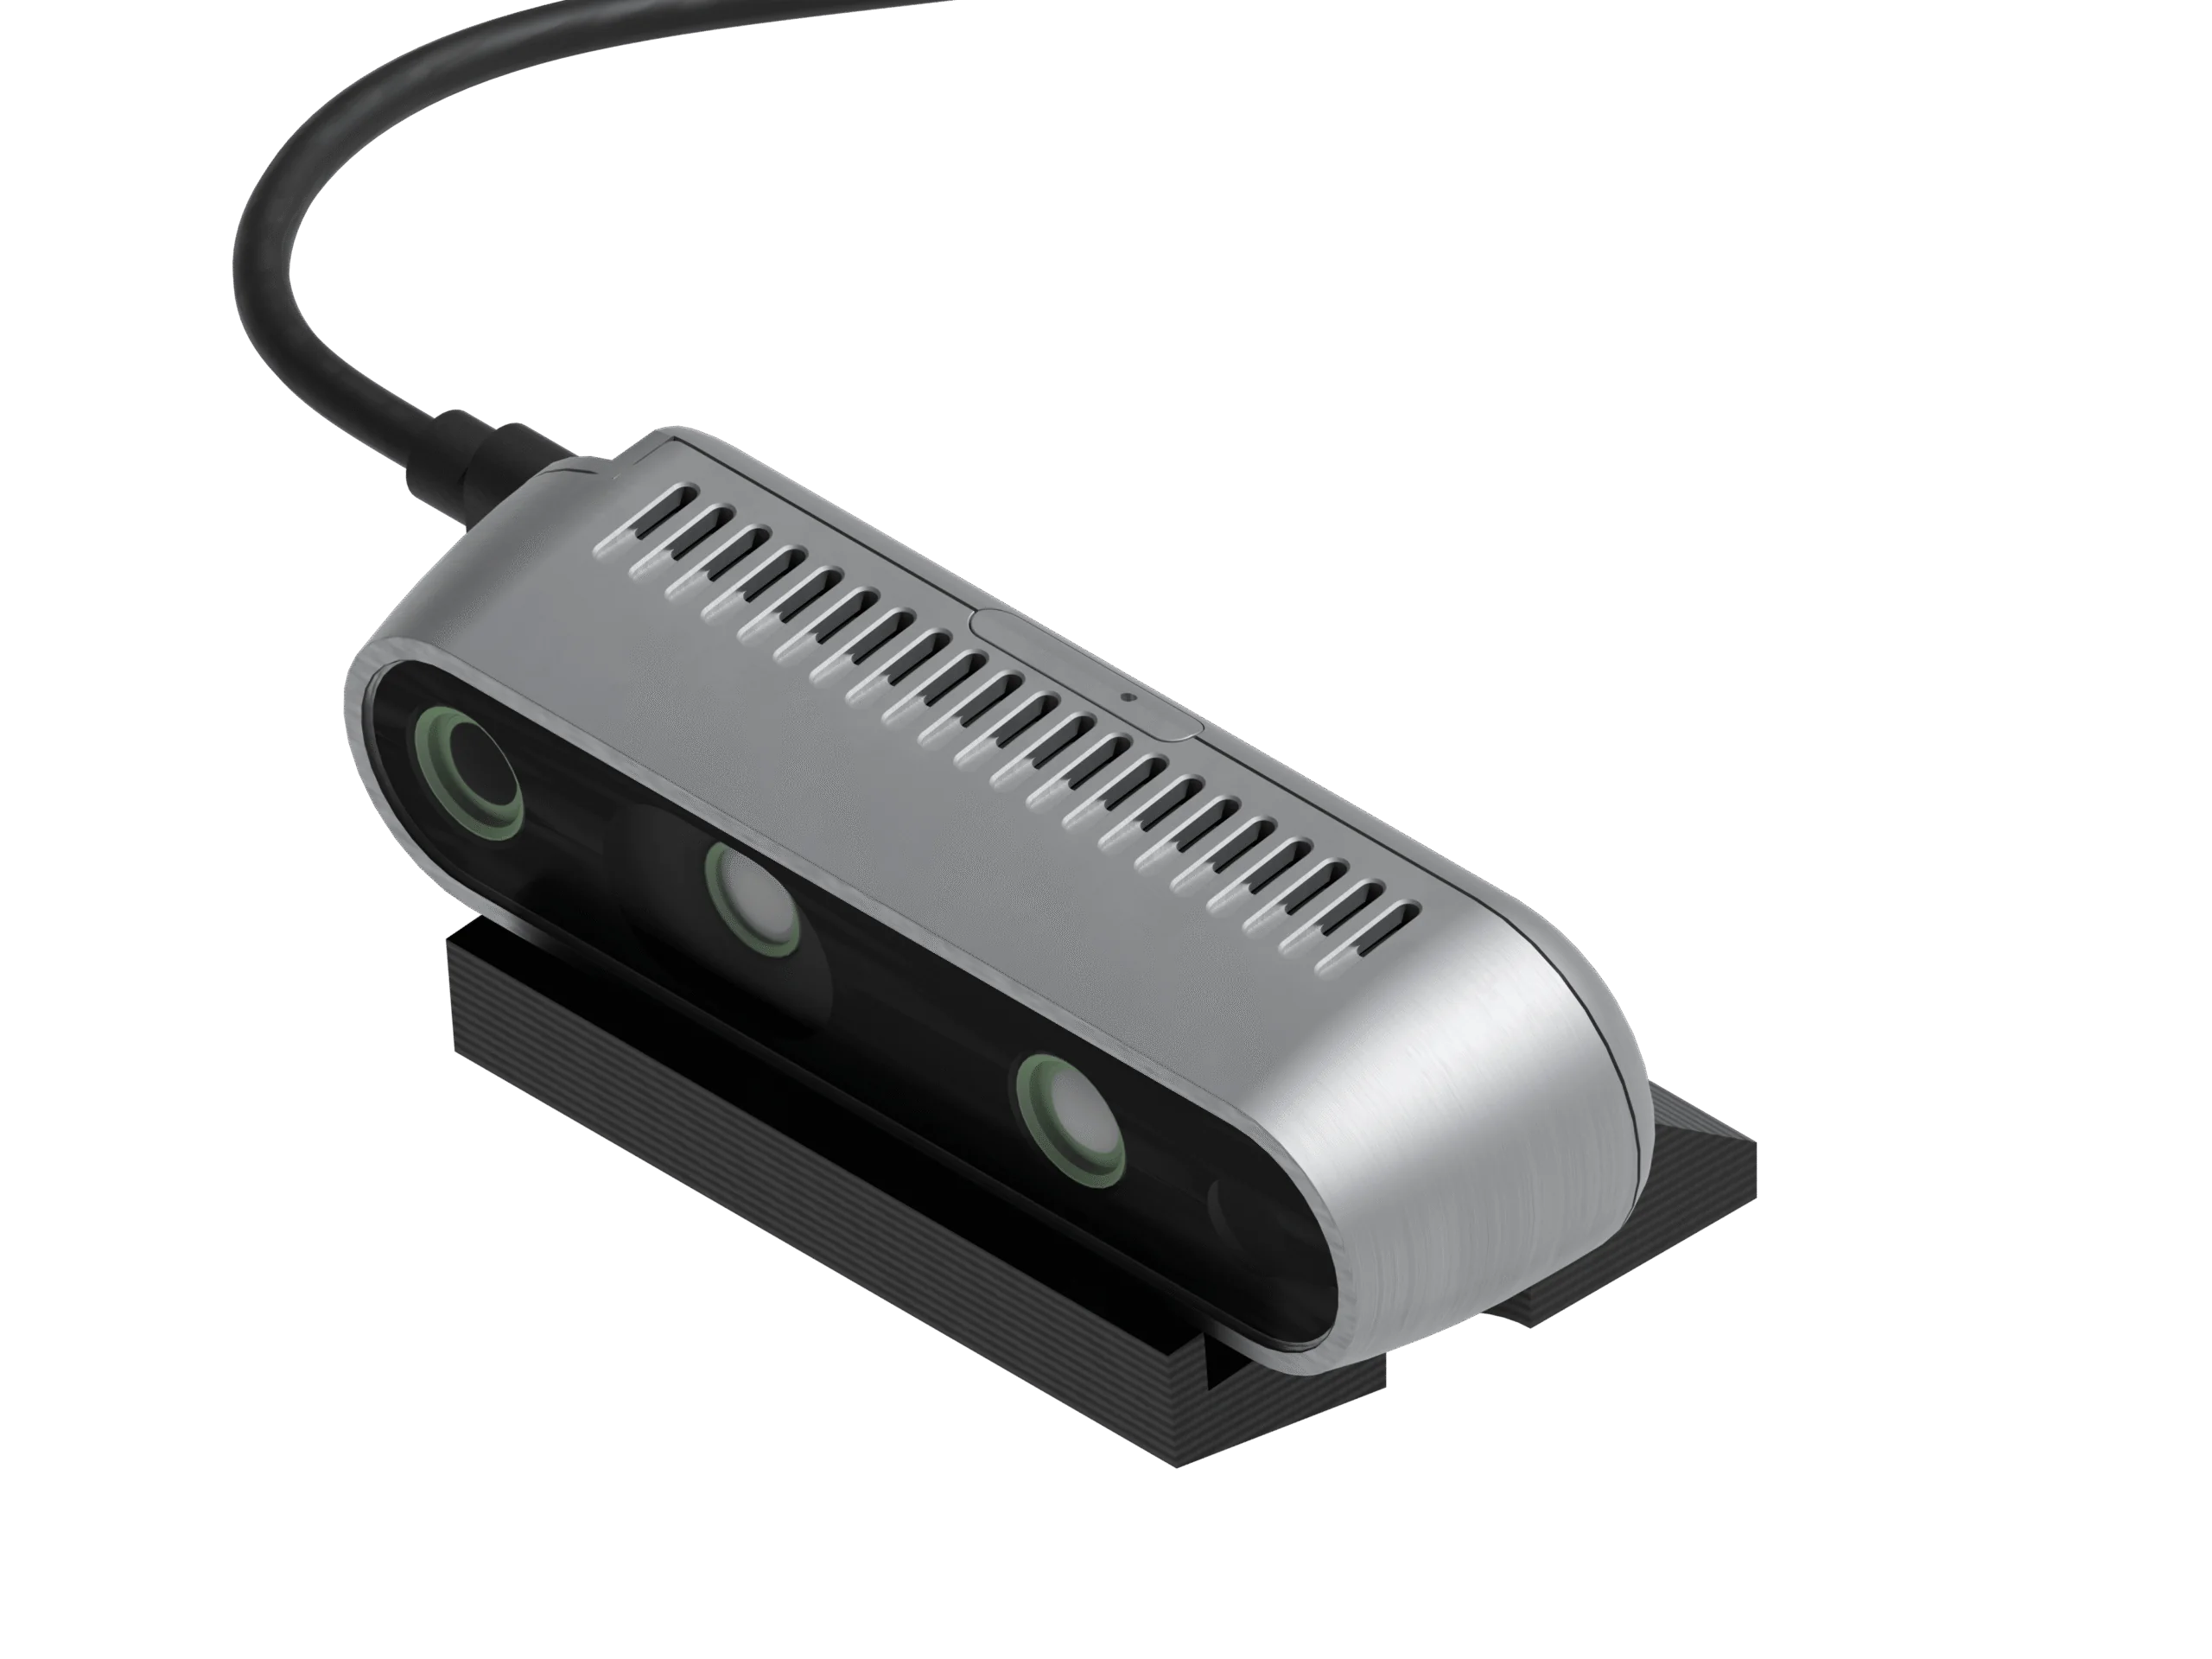
\includegraphics[width=1\linewidth]{subtex//images/camera.png}
    \caption{Realsense D435i Camera}
    \label{fig:camera}
\end{figure}




\subsection{Hardware Modifications}
The Lerobot SO-101, shown in Figure \ref{fig:unmodified lerobot arm} below, is an open source platform and was not immediately amenable for this application. Namely, the end-effector assembly and range of motion were not suited for bimanual tray lifting and translating. The team used Fusion 360 AutoDesk CAD to modify the design, and a Bambu X1E FDM 3D printer to manufacture the parts. 


\begin{figure} [h]
    \centering
    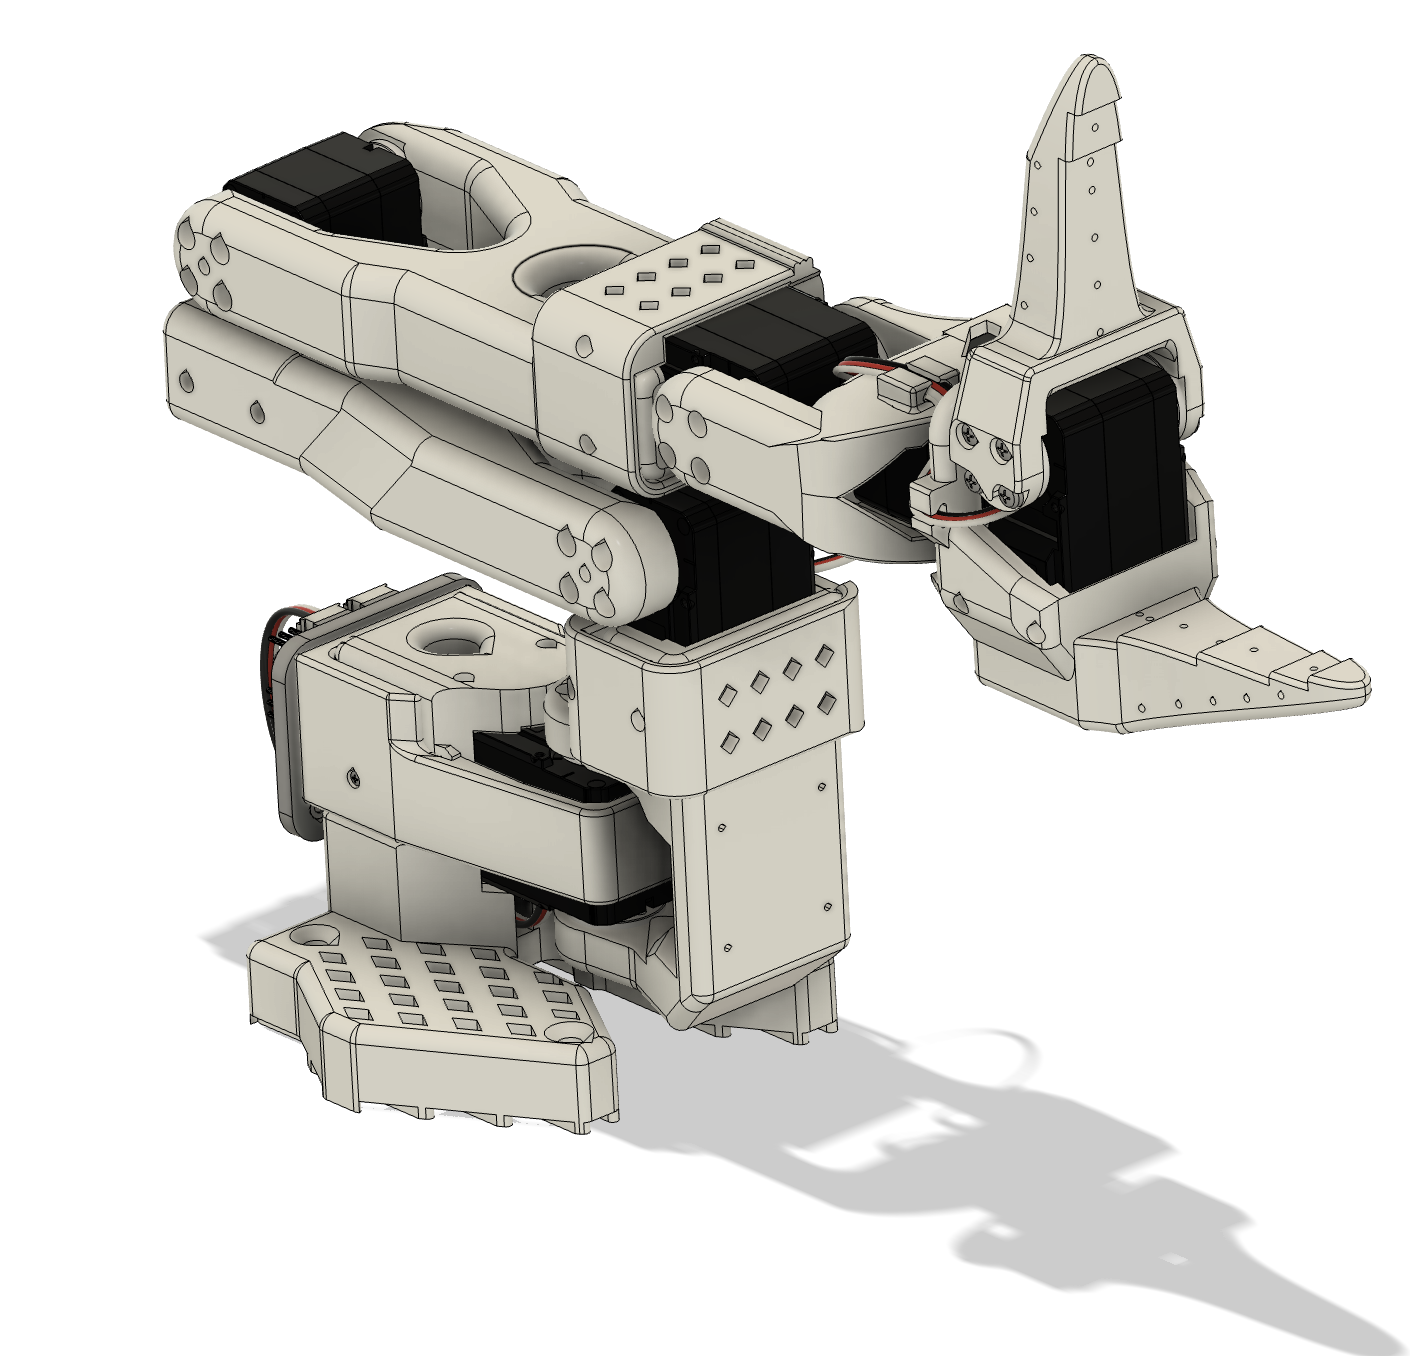
\includegraphics[width=1\linewidth]{subtex//images/original_lerobot.png}
    \caption{Unmodified Lerobot Arm}
    \label{fig:unmodified lerobot arm}
\end{figure}

The original "Finger-Tips" end-effector assembly shown in Figure \ref{fig:unmodified lerobot arm} was sub-optimal for our application. The swinging motion proved space-inefficient for a simplistic binary open-close program. The "Finger-Tips" were also originally printed in polylactic acid (PLA), a cost-effective but britle and unforgiving material for this application. Instead, another open source design \cite{so101grabcad} was used. This design features linearly translating grippers actuated through a gear and set of racks. A new servo casing and gear was designed to fit the STS3215 servo motor as shown in Figure \ref{fig:modified_end_effector_assembly}.




\begin{figure}[H]
    \centering
    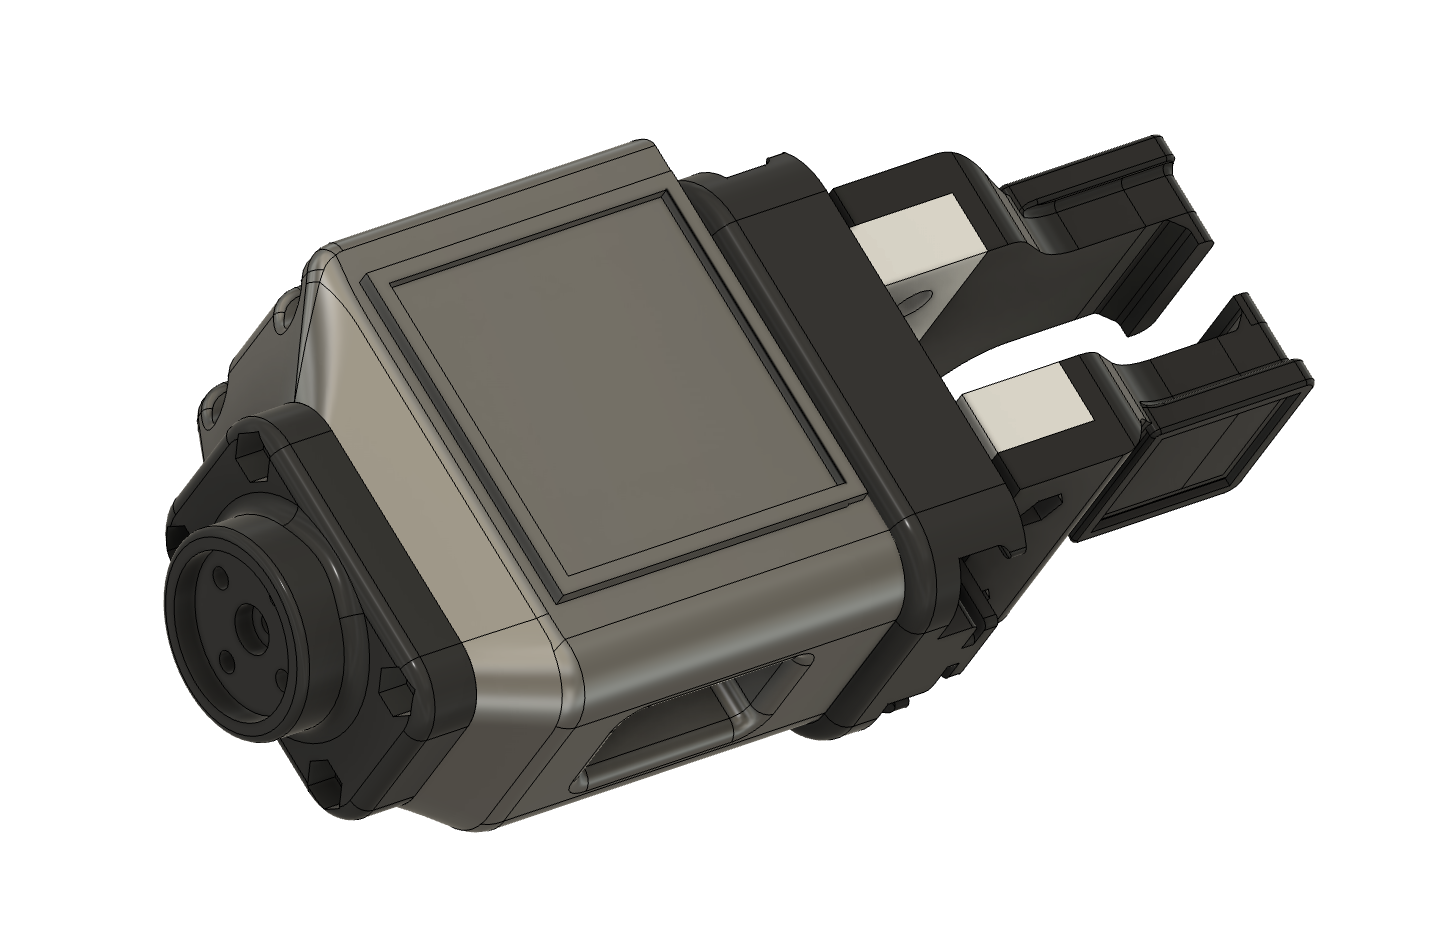
\includegraphics[width=1\linewidth]{subtex/images/gripper.png}
    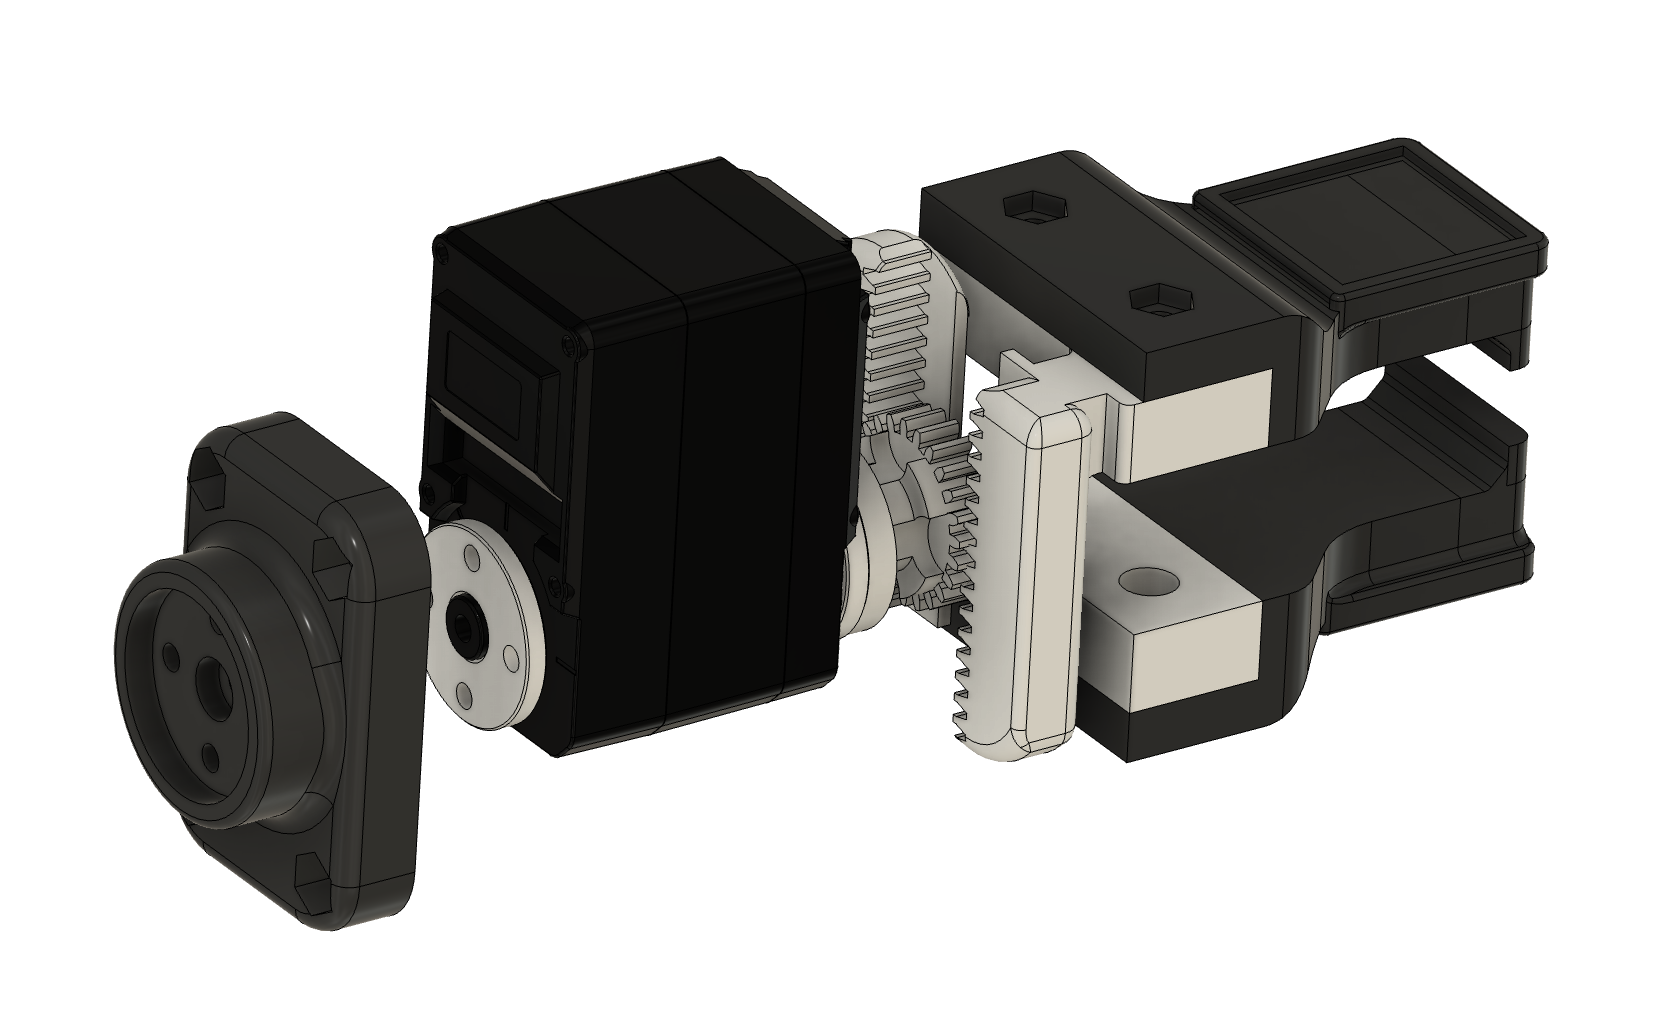
\includegraphics[width=1\linewidth]{subtex/images/exploded_end_effector.png}
    \caption{Modified End-Effector Assembly}
    \label{fig:modified_end_effector_assembly}
\end{figure}


The new design splits the individual end-effectors into two components, allowing for different materials. Thermoplastic polyurethane (TPU), a flexible filament, was used for the tips. This added flexibility was crucial in dampening excessive movement error during operation and program iteration. 

Another limiting design characteristic of the initial design was their range of motion when lifting the tray vertically at an extended distance. The robot end-effector would reach a ceiling and begin to rotate to achieve additional vertical range. This induced rotation would lead to task failure. To compensate, two modifications were made. First, the robot arm base was extended by 3 cm vertically, with the new design highlighting this modification shown in Figure \ref{fig:modified base picture}. Second, the "Bicep" arm, or lower robot arm, was also extended by 3 cm, again shown in Figure \ref{fig:bicep_picture}.

\begin{figure} [H]
    \centering
    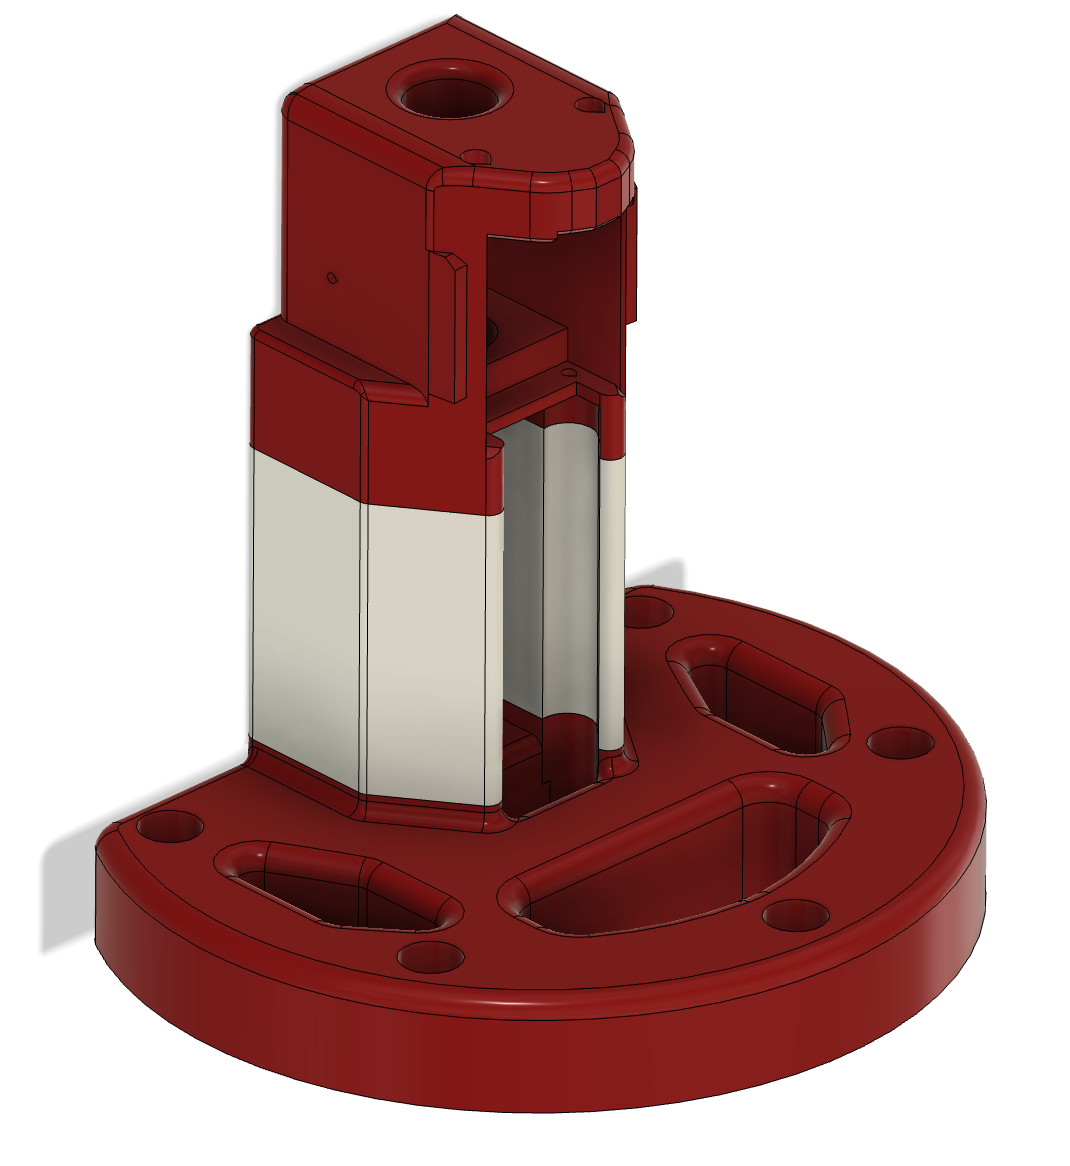
\includegraphics[width=1\linewidth]{subtex/images/base_modified.png}
    \caption{Modified Base}
    \label{fig:modified base picture}
\end{figure}

\begin{figure} [H]
    \centering
    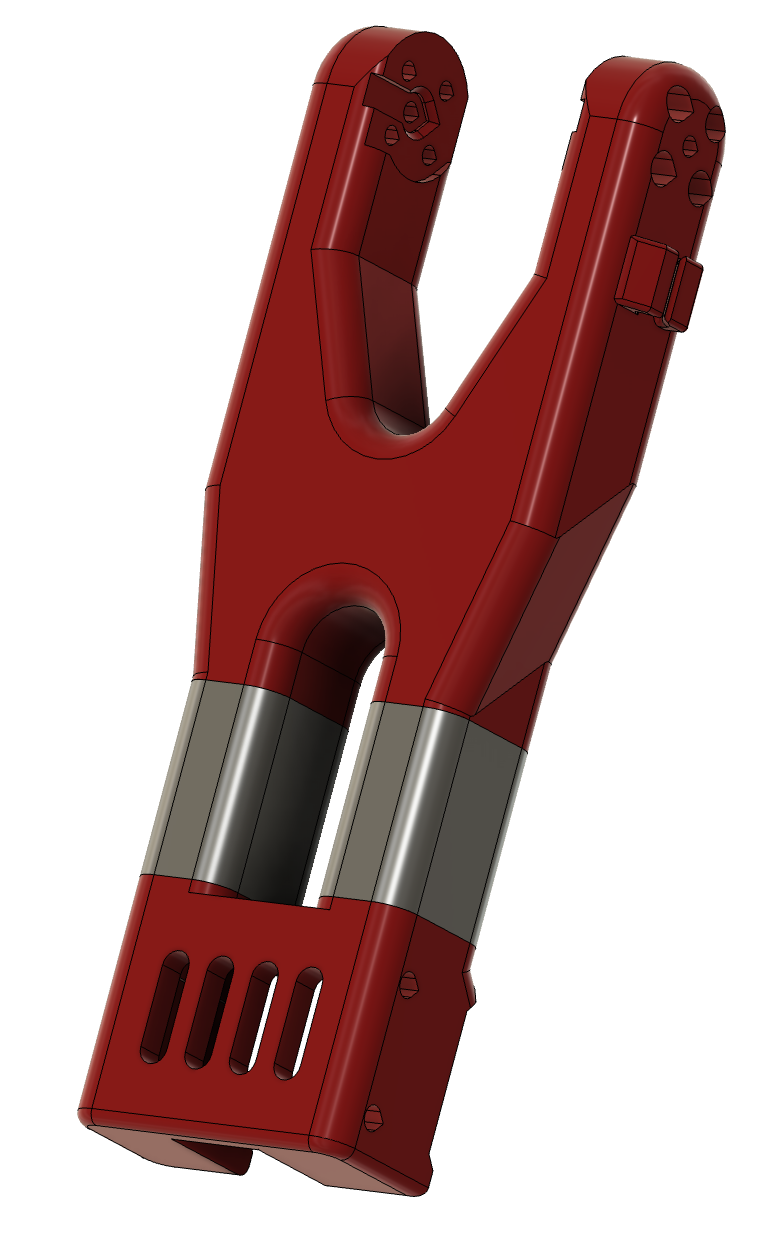
\includegraphics[width=.8\linewidth]{subtex/images/extended_bicep.png}
    \caption{Extended "Bicep" Arm}
    \label{fig:bicep_picture}
\end{figure}


\subsection{Tray}

The tray shown in Figure \ref{fig:tray} was designed from scratch. Printed from PLA, it features two AprilTag slots for 20 mm markers, as well as 10 mm wide handles raised 65 mm high. The tray itself is 150 mm in length and 75 mm in depth. While the tray design and assembly posed no significant problems towards the final task, a potential improvement, although less generalizable, would be to make a circular insert in the center to place the glass. This would prevent any lateral sliding in the case of jitter or small tilts.


\begin{figure} [H]
    \centering
    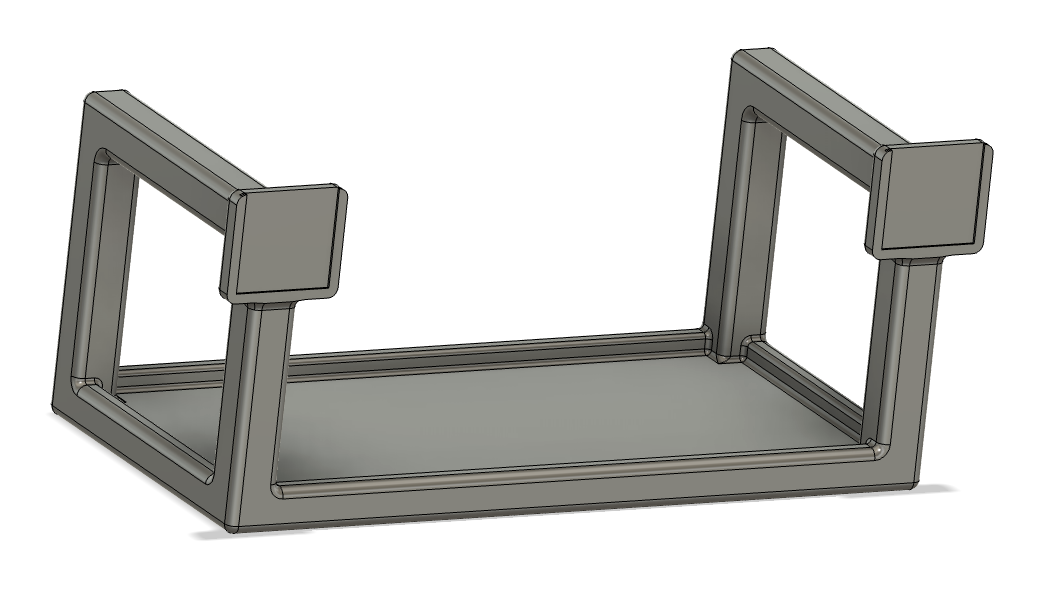
\includegraphics[width=1\linewidth]{subtex//images/tray.png}
    \caption{Custom Tray}
    \label{fig:tray}
\end{figure}




\section{Perception and Base-Frame Calibration}
\label{sec:perception}

This section covers the perception layer and how each arm turns a raw camera frame into 3D positions for control. The design is intentionally minimalistic. One ArUco detection (\texttt{cv2.aruco.ArucoDetector}~\cite{garrido2014aruco}) call per frame, followed by a \texttt{solvePnP} pose solver for each marker using its own physical size, generates 3D coordinates for each marker. There is no learning and no filtering beyond what OpenCV already provides. 

Each marker is assigned a semantic role via a \texttt{MarkerConfig} dataclass. These include \texttt{left\_base}, \texttt{right\_base},
\texttt{left\_gripper}, \texttt{right\_gripper}, \texttt{tray\_left}, and
\texttt{tray\_right}. The marker sizes were determined by where they sit. The base and gripper square AprilTag markers are 40 mm wide, which is large enough to track reliably all the way too the base. The two tray markers are 20 mm wide which is small enough to fit on the tray lip and large enough to remain detectable for the search and grab phases in the beginning. 


\subsection{From Pixels to Camera Frame}
For each detected marker, we recover its full 3D pose including position and orientation relative to the camera. This is a classical perspective-n-point (PnP) problem where given a set of 3D points whose layout is known, as well as their 2D pixel positions in the image, one must solve for the rigid transform that maps one to another.

The inputs are four detected marker corners represented as $\{(u_k, v_k)\}_{k=1}^{4}$, the camera matrix $K$, and the distortion
coefficients $\vec{d}$. We solved the perspective-n-point problem using \texttt{cv2.SOLVEPNP\_IPPE\_SQUARE}, which is built to handle coplanar square targets, against the symmetric object-frame corners
$(\pm s/2, \pm s/2, 0)$.


The output is then a rotation vector $\vec{r}$ in Rodriguez form, which is a compact 3-vector encoding of a rotation, and a translation $\vec{t}\in\mathbb{R}^3$. This is then combined into a homogeneous transform $T_{\text{cam}}^{\text{marker}}$, which is a representation telling where the marker is, in camera coordinates, used by the rest of the pipeline.

\subsection{Camera-to-Base Calibration}
\label{sec:calib}
The two arms sit at different positions and orientations across from each other on the table. Each arm has its own natural frame of reference offset from the other by the width of the table. The motion map for each arm, outlined in Section \ref{sec:motionmap}, is trained in its own base-frame coordinates, so before any task can be done, the system needs to know exactly how each arm base sits relative to the camera. An additional benefit of working in the base frame is that moving the entire setup to a new location only requires re-running the base-frame calibration.

For this, each arm's base carries a fixed 40 mm AprilTag. The system detects this tag for $N{=}30$ consecutive frames, and takes the average resulting rotation vectors and translations to produce an initial $T_{\text{cam}}^{\text{base}}$ per arm. By averaging over 30 frames, the per-frame jitter is suppressed while only adding one second of latency to startup. 

The averaged transform is almost correct, but not quite. Because the base tag is mounted by hand, its measured rotation comes back tilted by a degree or two from true vertical. Left uncorrected, that tilt propagated into every base-frame measurement downstream.

To fix this, the rotation is re-orthonormalized with explicit gravity alignment as a four-step process:
  \begin{enumerate}
      \item Project the camera's vertical axis onto each of the tag's three measured axes; whichever has the largest absolute projection is the axis that be vertical.
      \item Snap it to exactly vertical---this becomes the new $y$-axis.              
      \item Of the remaining two axes, take whichever is most aligned with the camera's depth direction, project it onto the horizontal plane, and call that the $z$-axis.
      \item Set the $x$-axis as $y \times z$ to close the right-handed frame.         
  \end{enumerate}                                           

  The result is a gravity-aligned $T_{\text{cam}}^{\text{base}}$ for each arm. This is a transform that places the arm's base with $y$ guaranteed to point straight up. Because both arms enforce the same vertical convention, their motion maps share common axes without ever requiring an external world frame.

\subsection{Cam-to-Base Transform Use at Runtime}
At every control tick, each marker's pose comes out of the perception module in camera coordinates. To make these coordinates usable, each one is converted into the calling arm's base frame with a single matrix multiplication, $T_{\text{base}}^{\text{cam}} {\vec{p}}$,
where ${\vec{p}}$ is the 4D lift of the 3D point. Its $(x, y, z)$ is padded with a trailing 1 to make a 4-length vector, the standard form for applying the 4×4 transform.

$T_\text{base}^\text{cam}$ is the inverse of the $T_\text{cam}^\text{base}$ computed in Section \ref{sec:calib}, precomputed once at startup so the runtime cost is just a single 4×4 multiply.

Because every visual measurement is pushed through the same transform, the rest of the pipeline never needs to track which marker is which. Tray markers, gripper markers, and any other point in the camera frame all arrive in the same base frame, and the motion map polynomial consumes them without further conversion.

\subsection{Per-Arm Asymmetry of Perception}
A side effect of using a shared camera with individual arm calibrations is that the two arms do not construct identical scene representations. Any calibration error in one transform becomes a bias in that arm's perceived workspace alone as it does not show up in the other arm's view.


This sounds like it could break coordination, since both arms reason about the same physical objects, but in practice it does not. The per-arm bias is on the order of millimeters, well below the 5–10 mm ArUco accuracy ceiling that bounds every other arm measurement. Also, the coordination algorithms of Section \ref{sec:coordination} are designed around inequalities and threshold comparisons that already absorb the noise.


\section{The Motion Map}
\label{sec:motionmap}

A central challenge in any robotic arm problem is inverse kinematics (IK): finding the positions of each motor in an arm to place the end effector at certain coordinates in 3D space with a certain orientation. In the case of the LeRobot SO-101 arm, only 5 of the 6 motors can contribute to this goal, as the last motor is used for the end effector. Thus, the arm is missing one DoF compared to the x-y-z and roll-pitch-yaw requirement. Traditional numerical solvers promise to converge to nearby solutions in this underactuated case, but they require precise measurements of each linkage in the arm in arbitrary coordinate frames, have slow iterative processes that might not be able to run at 30 Hz, and provide more functionality than is necessary for the goals of this project.

Instead, consider a motion map: a low-degree polynomial that takes a planar target $(x,z)$ and returns a 5-length vector of raw servo targets $\vec{q}\in\mathbb{R}^5$ (all arm joints except the gripper). The $y$ (height) coordinate is fixed during the sweep to a chosen hover height above the tray, so the map is
effectively a 2D $\!\to\!$ 5D regression.

\subsection{Motivation}
The polynomial form has three practical properties at once:
\begin{itemize}
  \item \textbf{O(1) evaluation.} The runtime control loop evaluates a degree-3 polynomial, not an iterative IK solver.
  \item \textbf{Smooth trajectories.} Polynomial output is
  continuous in the planar query, so continuous changes in goal
  position produce continuous joint motion without inverse-kinematics jitter or branch flips.
  \item \textbf{Ease of use} The map is extraordinarily easy to use once trained, requiring a single method call.
\end{itemize}

\subsection{Data Collection}
An operator manually sweeps each arm, with torque disabled, across the workspace while a real-time viewer shows (a) the live $y$ error against the target hover height and (b) a 40$\times$60 cell coverage grid at 5 mm resolution (to cover a 20$\times$30 cm area). Samples are only logged when the gripper marker is within $\pm5$\,mm of the target hover height. The operator aims for full grid coverage before stopping, but only about 70\% coverage was achieved in practice. A typical sweep produces $\sim$8k valid samples per arm in around 10 minutes. 

\subsection{Training the Polynomial}
\label{sec:mm-training}
Let $(\vec{x},\vec{q})$ be the collected
(position, joint-vector) pairs after per-cell
downsampling (keeping only 1 point per cell that has the lowest y-error). For each joint $j$ we fit a degree-3 polynomial by ridge regression on (mean and std dev) normalized features:
\begin{equation}
\label{eq:motion map fit}
  \vec{c}_j \;=\; (X^\top X + \alpha I)^{-1} X^\top \vec{q},
\end{equation}
with $\alpha = 10^{-3}$ for numerical stability and
$X=\bar{x}\bar{q}$ the matrix for mean-zero and unit-variance normalized inputs
$(\bar{x},\bar{q})$. 15\% of the points are held as a validation split which gave
RMSE around $3^\circ$ for most joints, but as high as $8^\circ$
for the wrist pan and roll joints that were not the main focus of the motion map (they just serve to keep the gripper oriented towards the camera).


Two empirical correction terms are slipped in at training time:
\begin{itemize}
  \item \textbf{Gravity offsets}: added to
  \texttt{shoulder\_lift}, \texttt{elbow\_flex}, and \texttt{wrist\_flex}
  before fitting to counteract the sag caused by hand-supporting the
  arm during recording.
  \item \textbf{Position offsets}:
  translations applied to the recorded (x,z)
  so that the polynomial learns to target the correct grasp point
  relative to the tray marker (ex. a 2 cm backward shift on both arms so the gripper lands on the middle of the handle, not directly on the marker
  itself).
\end{itemize}

\subsection{Runtime Evaluation}
At runtime, the motion map returns the joint target for a
desired planar query. Targets outside the recorded workspace bounds are rejected by the controller and result in the arm staying still rather than being extrapolated. Extrapolation was considered because it is a useful result of the polynomial nature of the motion map, however, implementation proved that the behavior of the arms was somewhat unpredictable as some joints quickly hit their physical rotation limits. There also was not much practical use case for work outside the mapped area, so extrapolation was scrapped.

\subsection{Feedback Correction}
Because the polynomial is fit before beginning, it will inherit any residual calibration or systematic error. We correct for this at runtime with a simple position-based visual servoing
loop~\cite{chaumette2006visual1} where we measure the planar error $\vec{e} = \vec{x}_{\text{target}} - \vec{x}_{\text{gripper}}$ and evaluate the polynomial at a shifted query $\vec{x}_{\text{target}} + \beta\vec{e}$ with $\beta=0.5$. This drives the gripper to the actual target rather than the open-loop estimate, closing the loop over time. This feedback correction has the side effect of sweeping the arm down and into the tray when the position error is large, so a raise-on-traverse correction was also added.

\subsection{Raise-on-Traverse}
To avoid sweeping the gripper through the tray when the planar error is large, the controller also adds a per-joint raise offset
proportional to $\|\vec{e}\|$, scaled by
\texttt{RAISE\_DIST\_SCALE\_M}~$=50$\,mm:
\begin{equation}
  q \;\mathrel{+}=\;
  \left(\frac{\|\vec{e}\|}{\texttt{RAISE\_DIST\_SCALE\_M}}\right)
  \Delta_{\text{raise}}
\end{equation}
This raises the arm by a delta for every 50 mm in position error that it currently has. This causes the arm to approach the target from above and settle down as $\|\vec{e}\|$ shrinks, rather than moving down into the tray during hover.

\section{Emergent Coordination via Shared Vision}
\label{sec:coordination}

This section presents the core contribution of the paper: a set of coordination primitives that let two independent arms cooperatively lift, translate, and lower a tray without any direct communication. All primitives share a common design principle, and are linked by a finite-state protocol (\cref{sec:protocol}) that both arms execute identically.

\subsection{Design Principle: Shared Observation as Shared State}
Much like humans tasked with moving a large object without communicating, two arms can still coordinate if, at every decision point, they have an observable representation of the information they would otherwise need to exchange. Our design uses three such proxies:

\begin{itemize}
  \item \textbf{Tray markers as shared position state.} Both arms see both tray markers. Their positions define what ``the
  tray is here'' means and their height difference defines
  what ``the tray is level'' means, for example.
  \item \textbf{Physical pre-move as a handshake signal.} Instead
  of sending a ``ready to lift'' message in a traditional sense, one arm physically lifts its side of the tray. 
  If the other arm knows to watch for that lift, the message has just been successfully passed.
  \item \textbf{The opposing gripper marker as a position reference
  during motion.} Tray markers are small (20 mm) and frequently
  drop during motion. The gripper markers are large (40 mm)
  and reliably visible. The follower in \cref{sec:translate} tracks
  the leader's gripper rather than the leader's tray marker during periods of faster motion.
\end{itemize}
With this message-passing framework, coordination is now enabled.


\begin{figure} 
    \centering
    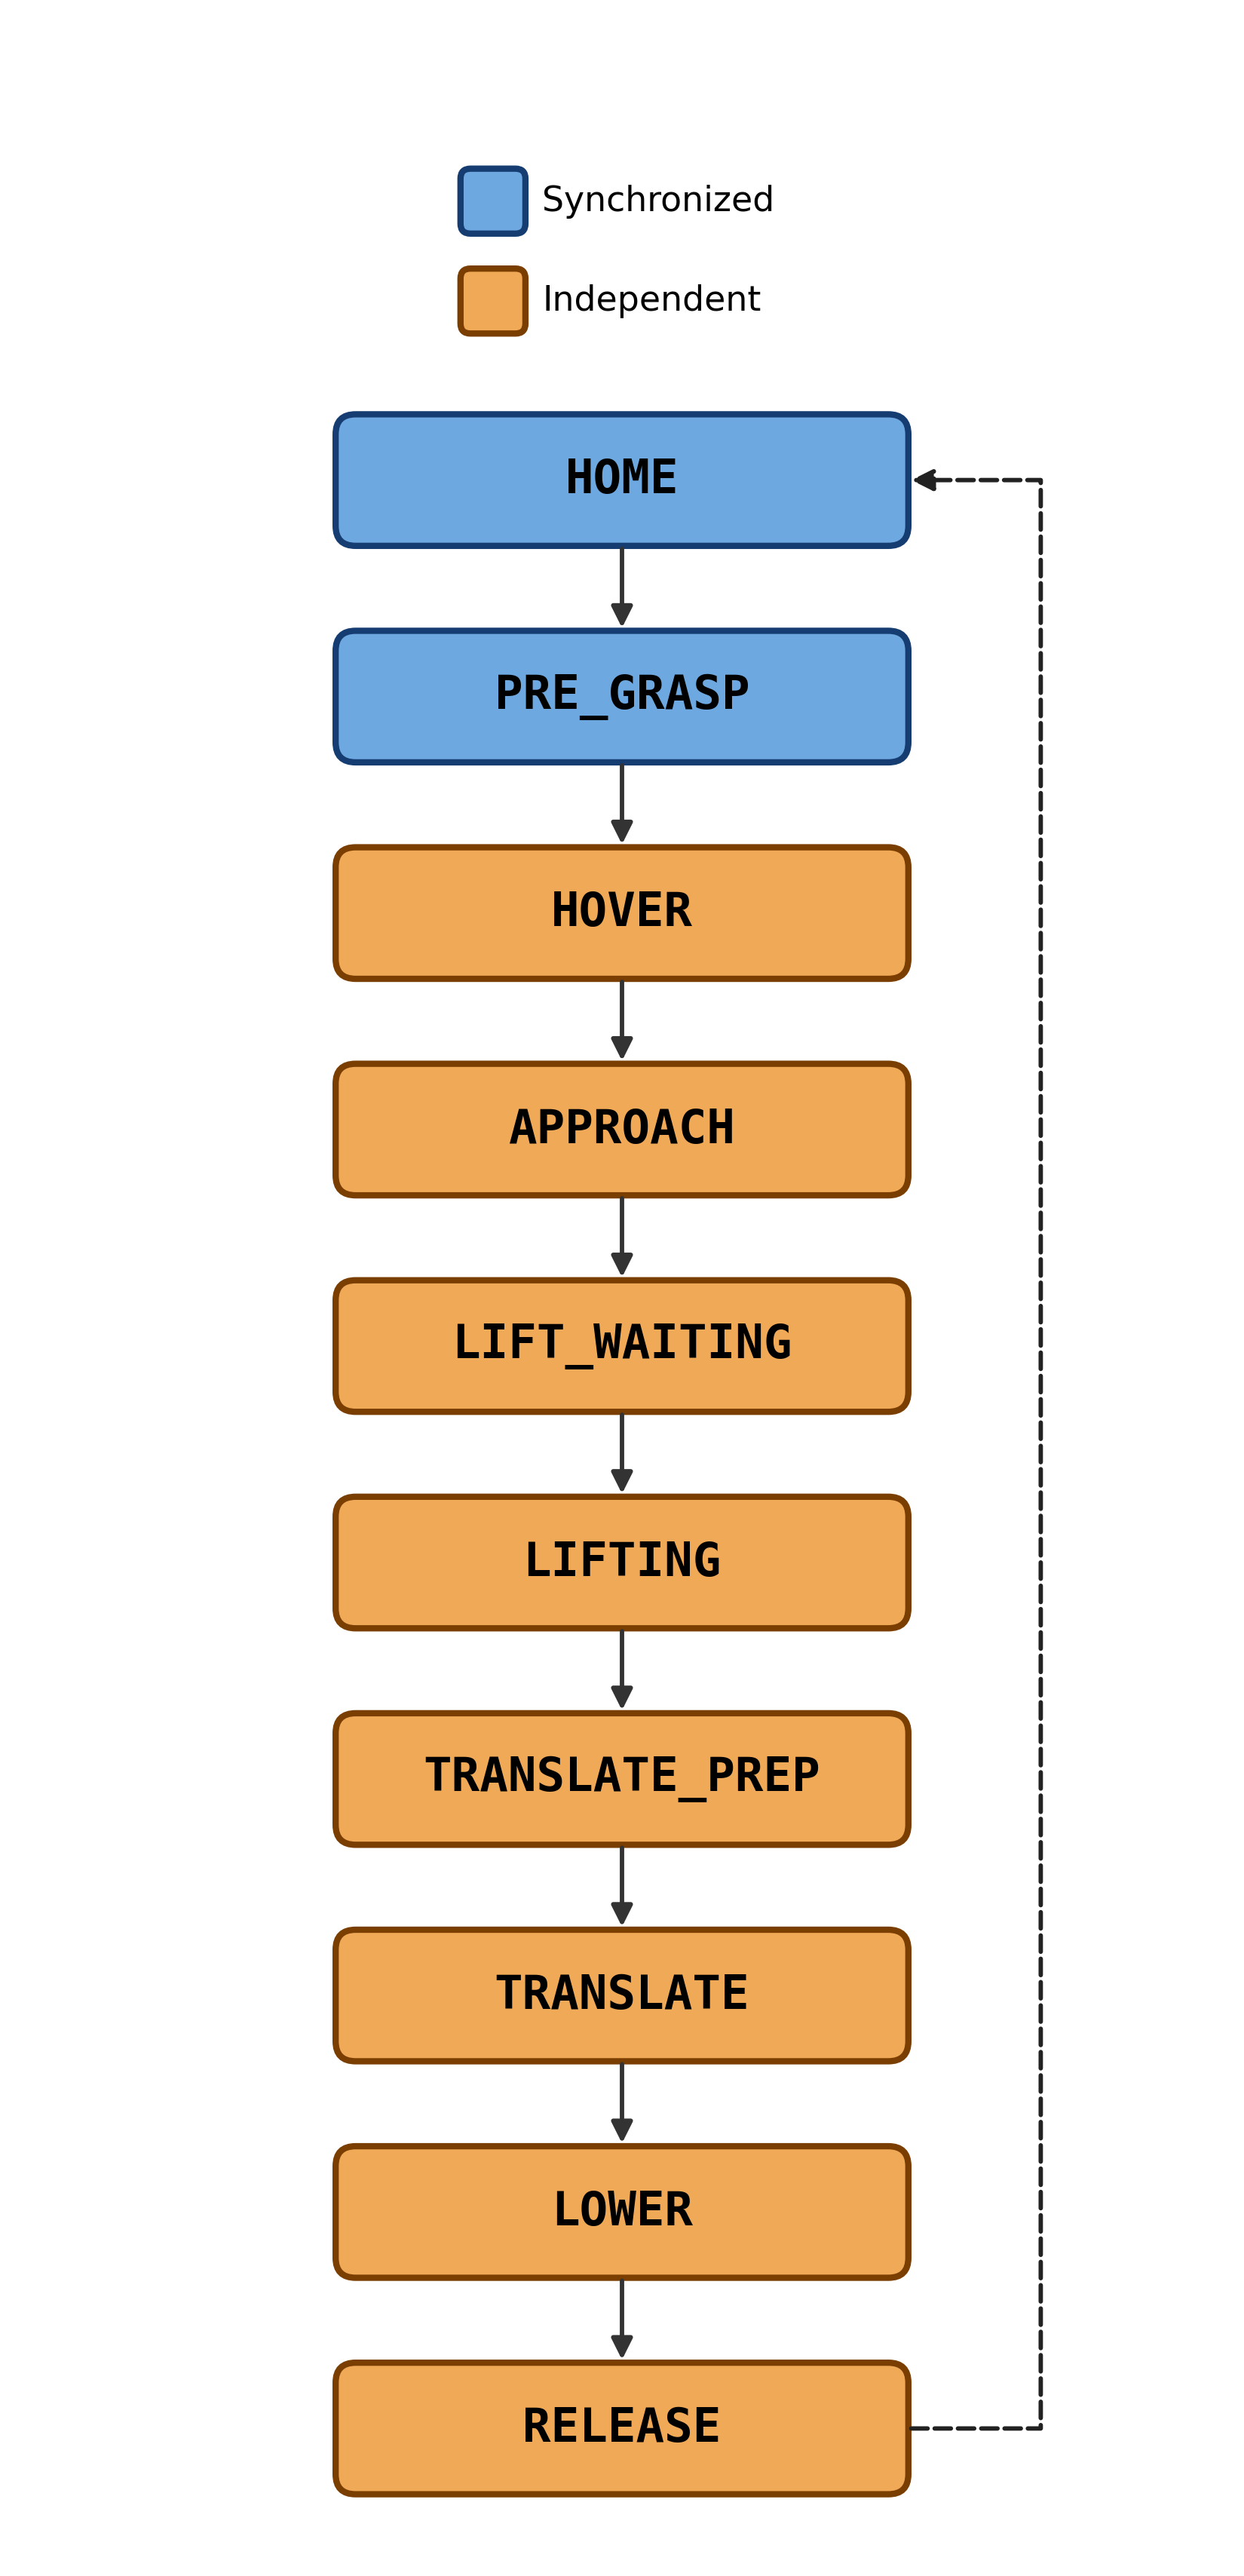
\includegraphics[width=1.16\linewidth]{subtex//images/figure9_state_diagram.png}
    \caption{Shared state-machine run by both arms. All states after \texttt{PRE\_GRASP} run independently. \texttt{PRE\_GRASP} serves only to move the arms into view of the camera, after which coordination must emerge.}
    \label{fig:fsm}
\end{figure}



\subsection{Finite-State Coordination Protocol}
\label{sec:protocol}
Both arms run the linear state machine shown in \cref{fig:fsm}. The first two states (\texttt{HOME} and \texttt{PRE\_GRASP}) are executed by the main thread with synchronized pre-planned moves that bring both arms to the center of the working area. From the \texttt{HOVER} phase onward, each arm runs the state machine in its own thread, issues its own commands, and transitions on its own visual events. The subsequent sections will detail each state and how the transitions to the next state are decided.


\subsection{Hover Convergence}
\label{sec:hover}
\cref{algo:hover} is the controller each arm runs during the
\texttt{HOVER} state. The arm servos over its own tray marker
through its motion map, with the gripper-to-target error fed back into the polynomial query as in \cref{sec:motionmap}. A transient raise proportional to $\|\vec{e}\|$ keeps the gripper \emph{above} the tray as it converges; a 30\% descent bias (subtracting $0.3\,\Delta_{\text{descent}}$ from the polynomial output) keeps the arm slightly above hover height when $\|\vec{e}\|\!\to\!0$, so the arm doesn't come into contact with the tray until it is time to grab. Importantly, the camera readings are converted into the base frame of each
arm first, as both motion maps work in that frame to allow generalization to new environments. A second note is that every position written to the servos is clamped under a maximum delta to decrease hardware stress.

\begin{algorithm} [h]
\caption{HOVER controller}
\label{algo:hover}
\begin{algorithmic}[1]
  \REQUIRE motion map $M$, my tray marker id, my gripper marker id,
           descent delta $\Delta_d$, base transform
           $T_{\text{base}}^{\text{cam}}$
  \STATE $\bar{\vec{x}} \gets \texttt{None}$;\ \ $n_{\text{conv}} \gets 0$
  \LOOP
    \STATE $F \gets \texttt{get\_frame}()$;\ \
           poses $\gets \texttt{detect}(F)$
    \STATE $\vec{x}_{\text{tray}}^{\text{cam}} \gets$
           \texttt{tray\_pose}(poses)
    \IF{$\vec{x}_{\text{tray}}^{\text{cam}}$ is \texttt{None}} \textbf{continue}
    \ENDIF
    \STATE $\vec{x}_{\text{tray}} \gets T_{\text{base}}^{\text{cam}}
           {\vec{x}}_{\text{tray}}^{\text{cam}}$
           \COMMENT{base frame transform}
    \STATE $\bar{\vec{x}} \gets
           \alpha\,\vec{x}_{\text{tray}} + (1\!-\!\alpha)\bar{\vec{x}}$
           \COMMENT{EMA, $\alpha{=}0.2$}
    \STATE $\vec{x}_{\text{tgt}} \gets \bar{\vec{x}} - \vec{o}_{\text{pos}}$
           \COMMENT{bake in position offset}
    \STATE $\vec{x}_{\text{grip}} \gets T_{\text{base}}^{\text{cam}}$\,
           \texttt{gripper\_pose}(poses)
    \STATE $\vec{e} \gets \vec{x}_{\text{tgt}} - \vec{x}_{\text{grip}}$
    \STATE $\vec{q} \gets M(\bar{\vec{x}} + \beta\vec{e})$
           \COMMENT{feedback-corrected query}
    \STATE $\vec{q} \gets \vec{q} - 0.3\,\Delta_d$
           \COMMENT{absolute height increase}
    \STATE $\vec{q} \gets \vec{q} + (\|\vec{e}\|/r_0)\,\vec{\Delta}_{\text{raise}}$
           \COMMENT{error-driven height increase}
    \STATE clip per-step $|\Delta \vec{q}|\le q_{\max}$,\ write $\vec{q}$
    \IF{$\|\vec{e}\| < \tau_c$} 
    $n_{\text{conv}} \mathrel{+}= 1$
            \COMMENT{require 3 frames to break}
    \ELSE\ $n_{\text{conv}} \gets 0$ \ENDIF
    \IF{$n_{\text{conv}} \ge 3$} \textbf{break} \ENDIF
  \ENDLOOP
\end{algorithmic}
\end{algorithm}

An exponential moving average (EMA) with $\alpha{=}0.2$ smooths the tray position to suppress marker jitter. Convergence is declared when $\|\vec{e}\| <
\texttt{CONVERGENCE\_THRESHOLD\_M}=20$\,mm persists for
\texttt{CONVERGENCE\_READINGS}~$=3$ consecutive frames, guarding against a single lucky measurement. This convergence is the trigger that transitions each arm to the next state. In practice, hovering and converging resulted in the largest desyncronization between arms, so regaining that synchronization in the next phases is essential.


\subsection{Approach: Descend Until Vertically Close}
From \texttt{HOVER}, the arm opens its gripper and descends at a fixed rate (\texttt{LIFT\_STEP\_FRACTION}~$=3\%$ of the descent delta every 20 ms), accumulating commanded joint targets rather than applying a delta after each step, which results in movements too small to bypass the servo dead-band. Descent stops when the vertical distance between the tray marker and the gripper marker falls below \texttt{GRASP\_PROXIMITY\_M}~$=86$\,mm, which is the geometric distance between the gripper marker and tray marker when
the gripper just barely reaches the handle. The gripper closes, and the arm transitions to \texttt{LIFT\_WAITING}. This state has no checks for coordination, so any 
timing problems propagating from the hover are still present.

\subsection{Nudge-Lift Handshake}
\label{sec:nudge}
\cref{algo:nudge} describes the nudge-lift, a key coordination move. If either arm lifts alone, the tray tilts and the task fails. If each arm lifts as soon as it arrives, we rely on the previous states to have been synchronized, which almost never happened in practice. The nudge-lift handshake replaces an explicit message with a simple small physical commitment whre each arm pulls its side of the tray upward by \texttt{NUDGE\_FRACTION}$\,\cdot\,\Delta_{\text{descent}}=40\%$ of a descent delta. Each arm then watches the opposite tray
marker and waits for it to have risen by
\texttt{TAG\_RISE\_THRESHOLD\_M}~$=3$\,mm relative to a baseline position captured during \texttt{PRE\_GRASP}. 

Two properties of this algorithm are worth noting. First, the handshake is symmetric in that both arms do the same thing and wait on the same thing. The protocol has no leader-follower role. Second, the handshake cannot false-positive. If one gripper failed to close on the tray, its side of the tray will never move, so neither arm proceeds. This results in a failure
of the goal, but at least the water won't be spilled and the arms will stop. When an arm detects the other arm's perturbation lift (and has already completed it's own lift), it transitions to the next state.


\begin{algorithm} [h]
\caption{Nudge-lift (physical message passing)}
\label{algo:nudge}
\begin{algorithmic}[1]
  \REQUIRE descent delta $\Delta_d$, opposing tray key $k_{\text{other}}$,
           baseline height $y_{\text{other},0}$,
           thresholds $\tau_r=3$\,mm,\ nudge fraction $\eta_n=0.4$
  \STATE Nudge: smooth move, $-\eta_n\Delta_d$ in joint space
  \LOOP
    \STATE $F \gets \texttt{get\_frame}()$;\ poses $\gets \texttt{detect}(F)$
    \STATE $y_{\text{other}} \gets $
           \texttt{tray\_poses}(poses)$[k_{\text{other}}]\,.y$
    \STATE $\texttt{rise} \gets y_{\text{other},0} - y_{\text{other}}$
           \COMMENT{camera $y$ down; rise = $-\Delta y$}
    \IF{$\texttt{rise}\ge \tau_r$} \textbf{break} \ENDIF
  \ENDLOOP
\end{algorithmic}
\end{algorithm}

\subsection{Tilt-Aware Synchronized Lift}
\label{sec:lifting}
Once the handshake completes, both arms transition to \texttt{LIFTING} simultaneously (within one frame of each other, bounded by the rise-detection latency). It is possible that a hard-coded lift would be viable here because the arms are well coordinated at this point, but this poses no merit and a synchronized lift would guarantee success. 


Therefore, we implement coordination as a sort of self-throttling. At each \texttt{LIFTING} step, each arm measures both tray markers' rise from baseline and advances its own target upward only if its own side is lower than the other:
\begin{equation}
\label{eq:lift-gate}
  \text{step this tick} \iff
  (\text{my rise}) \le (\text{other rise}).
\end{equation}
This is a one-line rule with important properties. If the two arms move identically, both step every tick and ascend together. If one arm leads, it stops stepping until the other catches up. If one arm's servos stall transiently, the other naturally pauses. Neither arm ever needs to know which arm is leading. Both arms see the same heights and make the same local decision, and the tray stays level to within the measurement noise. Another important part of this algorithm differentiating it from predecessors is that it uses an explicit sleep for 20 ms every loop. This prevents stacking the same joint delta extremely quickly, as everything in this loop is quick to compute.

Once an arm's own rise reaches \texttt{LIFT\_HEIGHT\_M}~$=60$\,mm, it stops looping and proceeds to \texttt{TRANSLATE\_PREP}. Because the arms are so synchronized during the lift, this transition usually happens at the same time, offset by only a few frames. This culminates in global synchronized from visual cues alone.

\begin{algorithm} [h]
\caption{Tilt-aware LIFTING}
\label{algo:lift}
\begin{algorithmic}[1]
  \REQUIRE per-step lift $\vec{\delta}=-\,\texttt{LIFT\_STEP\_FRACTION}\,\Delta_d$,
           target rise $H$, my tray key $k_m$, other key $k_o$,
           baselines $y_{m,0}, y_{o,0}$
  \STATE $\vec{q}^\star \gets $ \texttt{read\_joints()}
  \LOOP
    \STATE poses $\gets \texttt{detect}(\texttt{get\_frame}())$
    \STATE $r_m \gets y_{m,0}-\text{poses}[k_m].y$;\ \
           $r_o \gets y_{o,0}-\text{poses}[k_o].y$
    \IF{$r_m \ge H$} \textbf{break} 
    \ENDIF
    \IF{$r_m \le r_o$}
       \STATE $\vec{q}^\star \gets \vec{q}^\star + \vec{\delta}$;\ \
              \texttt{write\_joints}($\vec{q}^\star$)
    \ENDIF
    \STATE \texttt{sleep}(20\,ms)
  \ENDLOOP

\end{algorithmic}
\end{algorithm}

\subsection{Leader--Follower Translation}
\label{sec:translate}
The tray is now lifted and level. The forward translation must move both grasp points through the same horizontal trajectory at the same speed, or the tray pivots about whichever point lags. Because the grippers must remain spaced by the tray width, the simplest plan to have both arms sweep an interpolation from the current position to a goal will not work. Coordination is required.

We instead utilize an asymmetric leader-follower scheme. Before
\texttt{TRANSLATE} begins, a single observation measures the
base-frame offset from the left gripper marker to the
right tray marker:
\begin{equation}
\label{eq:offset}
  \vec{o} \;=\; \vec{x}_{\text{tray}_r}^{\text{base}_r}
           - \vec{x}_{\text{grip}_l}^{\text{base}_r},
\end{equation}
where both quantities are expressed in the right arm's base
frame. Because the tray is rigid and level after \cref{algo:lift},
this offset is a constant over the translation. It encodes the
tray width plus whatever small offset the grippers impose.

During translation, the left arm acts as the \textbf{leader}. It plans an interpolation in $(x,z)$ from its current
position to a pre-recorded destination way-point, evaluates its motion map at each intermediate query, and writes to the joints. It is essential that this interpolation happens in 3D space and uses the motion map because the simpler linear interpolation in joint space creates less-intuitive curved trajectories that sometimes resulted in infeasible follower tracking or tray bending. The right arm acts as the \textbf{follower}: each tick, it reads the left gripper marker (large, reliable), transforms it into its own base frame, and adds the offset $\vec{o}$ to obtain its target. Evaluating the right-arm motion map at this target yields the follower's joint command. An EMA ($\alpha=0.1$) smooths the
target to dampen marker noise.

As presented, this algorithm resulted in large jump discontinuities between the top of the lift and the beginning of the (somewhat) smooth slide. To remedy this, we implemented
a \texttt{TRANSLATE\_PREP} phase as mentioned in the previous section. This phase happens immediately after the lift, and consists of only an interpolation between the current position and the first motion map query result in joint space over one second. This serves to smooth the jump from joint space
onto the motion map. After the one second, each arm immediately transitions to \texttt{TRANSLATE}.
Conceptually, this phase should not be necessary, but in practice we concluded that our implementation of
\texttt{find\_closest\_coords}, a brute-force motion map method that finds coordinates nearby to the inputted joint positions by checking error at all of the points, results in jumps that are larger than we had hoped. Our hypothesis is that because we are finding nearby points in joint space, the nearest point might be something that is a close match for a few of the motors, resulting in low error, but far for one or two of the motors causing a large swing. \texttt{TRANSLATE\_PREP} solves this issue.

The key observation coordination-wise is that the follower never needs to know the leader's plan. Whatever trajectory the leader executes, the follower tracks it through
$\vec{o}$, because the leader's gripper position encodes its
intent with zero latency via the shared camera. The full algorithm is presented in \cref{algo:translate}.

\begin{algorithm} [h]
\caption{TRANSLATE: leader and follower}
\label{algo:translate}
\begin{algorithmic}[1]
  \STATE {\bfseries Pre:} measure
         $\vec{o} \gets \vec{x}_{\text{tray}_r} -
          \vec{x}_{\text{grip}_l}$ once
  \STATE // \emph{Leader (side = left):}
  \STATE $\vec{x}_s \gets$ current tray $(x,z)$
  \STATE $\vec{x}_d \gets$ \texttt{find\_closest\_coords}($M_l$,
         way-point$_{\text{left}}$)
  \FOR{$k=1,\dots,n_{\text{steps}}$}
    \STATE $\vec{x}_k \gets \vec{x}_s + smooth(\vec{x}_d-\vec{x}_s)$
    \STATE $\vec{q} \gets M_l(\vec{x}_k) + \vec{h}_{\text{trim}}$;\
           \texttt{write\_joints}($\vec{q}$)
    \STATE \texttt{sleep}(33\,ms)
  \ENDFOR
  \STATE // \emph{Follower (side = right):}
  \FOR{$k=1,\dots,n_{\text{steps}}$}
    \STATE $\vec{x}_g \gets T_{\text{base}_r}^{\text{cam}}\,
           \texttt{gripper\_pose}_\text{left}(\text{poses})$
    \STATE $\vec{x}_t \gets \vec{x}_g + \vec{o}$
    \STATE $\bar{\vec{x}}_t \gets
           \alpha_f\vec{x}_t+(1\!-\!\alpha_f)\bar{\vec{x}}_t$
           \COMMENT{EMA, $\alpha_f{=}0.1$}
    \STATE $\vec{q} \gets M_r(\bar{\vec{x}}_t) + \vec{h}_{\text{trim}}$;
           \ \texttt{write\_joints}($\vec{q}$)
    \STATE \texttt{sleep}(33\,ms)
  \ENDFOR
\end{algorithmic}
\end{algorithm}

\subsection{Tilt-Aware Lowering}
\label{sec:lower}
Lowering is mostly symmetric to the lift, and has similar failure modes, but the motion is opposite. We protect against the tilting failures with a tilt-pause rule (\cref{algo:lower}): at each tick, the arm pauses its descent if
its own tray marker is physically lower than the other's by more
than \texttt{TILT\_PAUSE\_THRESHOLD\_M}~$=5$\,mm, letting the
higher side catch up before both sides continue down. The rule is identical on both arms which, like \eqref{eq:lift-gate}, naturally synchronizes two independent descenders. One thing to note about this algorithm is the use of a discrete counter variable to limit how long the loop can run for. This is because we need to guarantee that both arms will eventually release the tray to finish the movement. This remedies an issue
in which the arms would lower the tray to the table, but continue to hold it waiting to lower further. The parameter was tuned such that the arms never let go of the tray too early.

\begin{algorithm} [t]
\caption{Tilt-aware LOWER}
\label{algo:lower}
\begin{algorithmic}[1]
  \REQUIRE lower destination $\vec{q}_d$, duration $T$,
           threshold $\tau_t=5$\,mm
  \STATE $\vec{q}_s \gets$ \texttt{read\_joints()};\ \ $k \gets 0$
  \WHILE{$k < n$}
    \STATE poses $\gets \texttt{detect}(\texttt{get\_frame}())$
    \STATE $\texttt{tilt} \gets
            \text{poses}[k_m].y - \text{poses}[k_o].y$
            \COMMENT{cam $y$ down}
    \IF{$\texttt{tilt} > \tau_t$}
      \STATE // my side lower: wait
      \STATE \texttt{sleep}(20\,ms);\ \textbf{continue}
    \ENDIF
    \STATE $\vec{q} \gets \vec{q}_s + smooth(\vec{q}_d-\vec{q}_s)$;
           \ \texttt{write\_joints}($\vec{q}$)
    \STATE $k \gets k+1$;\ \texttt{sleep}(20\,ms)
  \ENDWHILE
\end{algorithmic}
\end{algorithm}

\subsection{Release and Return}
On \texttt{RELEASE}, each arm opens its gripper and performs an interpolated move to a pre-recorded way-point that is directly above the tray to ensure clearance, then to the home way-point. No coordination is required here as the tray is static on the table. Now the task has been completed.

\section{Experimental Evaluation}
\label{sec:results}

\subsection{Experimental Setup}

As described in Section \ref{sec:system}, all results were collected on the physical dual-SO-101 setup. The tray carried a glass filled with water, resting on the tray center. Each trial began with the arms near \texttt{HOME} and the tray placed in a varied, but central position within the recorded workspace.

\subsection{End-to-End Success Rate \& Failure Modes}

A set of 50 trials were run using our algorithm, during which the failures at each phase were noted. Figure \ref{fig:failure rate per phase} illustrates the total failures per phase out of total number of trials that made it to that phase. Out of the 50 trails, the arms made it back to the \texttt{HOME} position successfully 37 times, which is a 74\% success rate. A clear pattern was established where failures concentrate at the start of the trajectory when the arms must locate and attach to the tray, vanish through the middle of the lift and translate, and return briefly during \texttt{LOWER}. 

\begin{figure} [H]
    \centering
    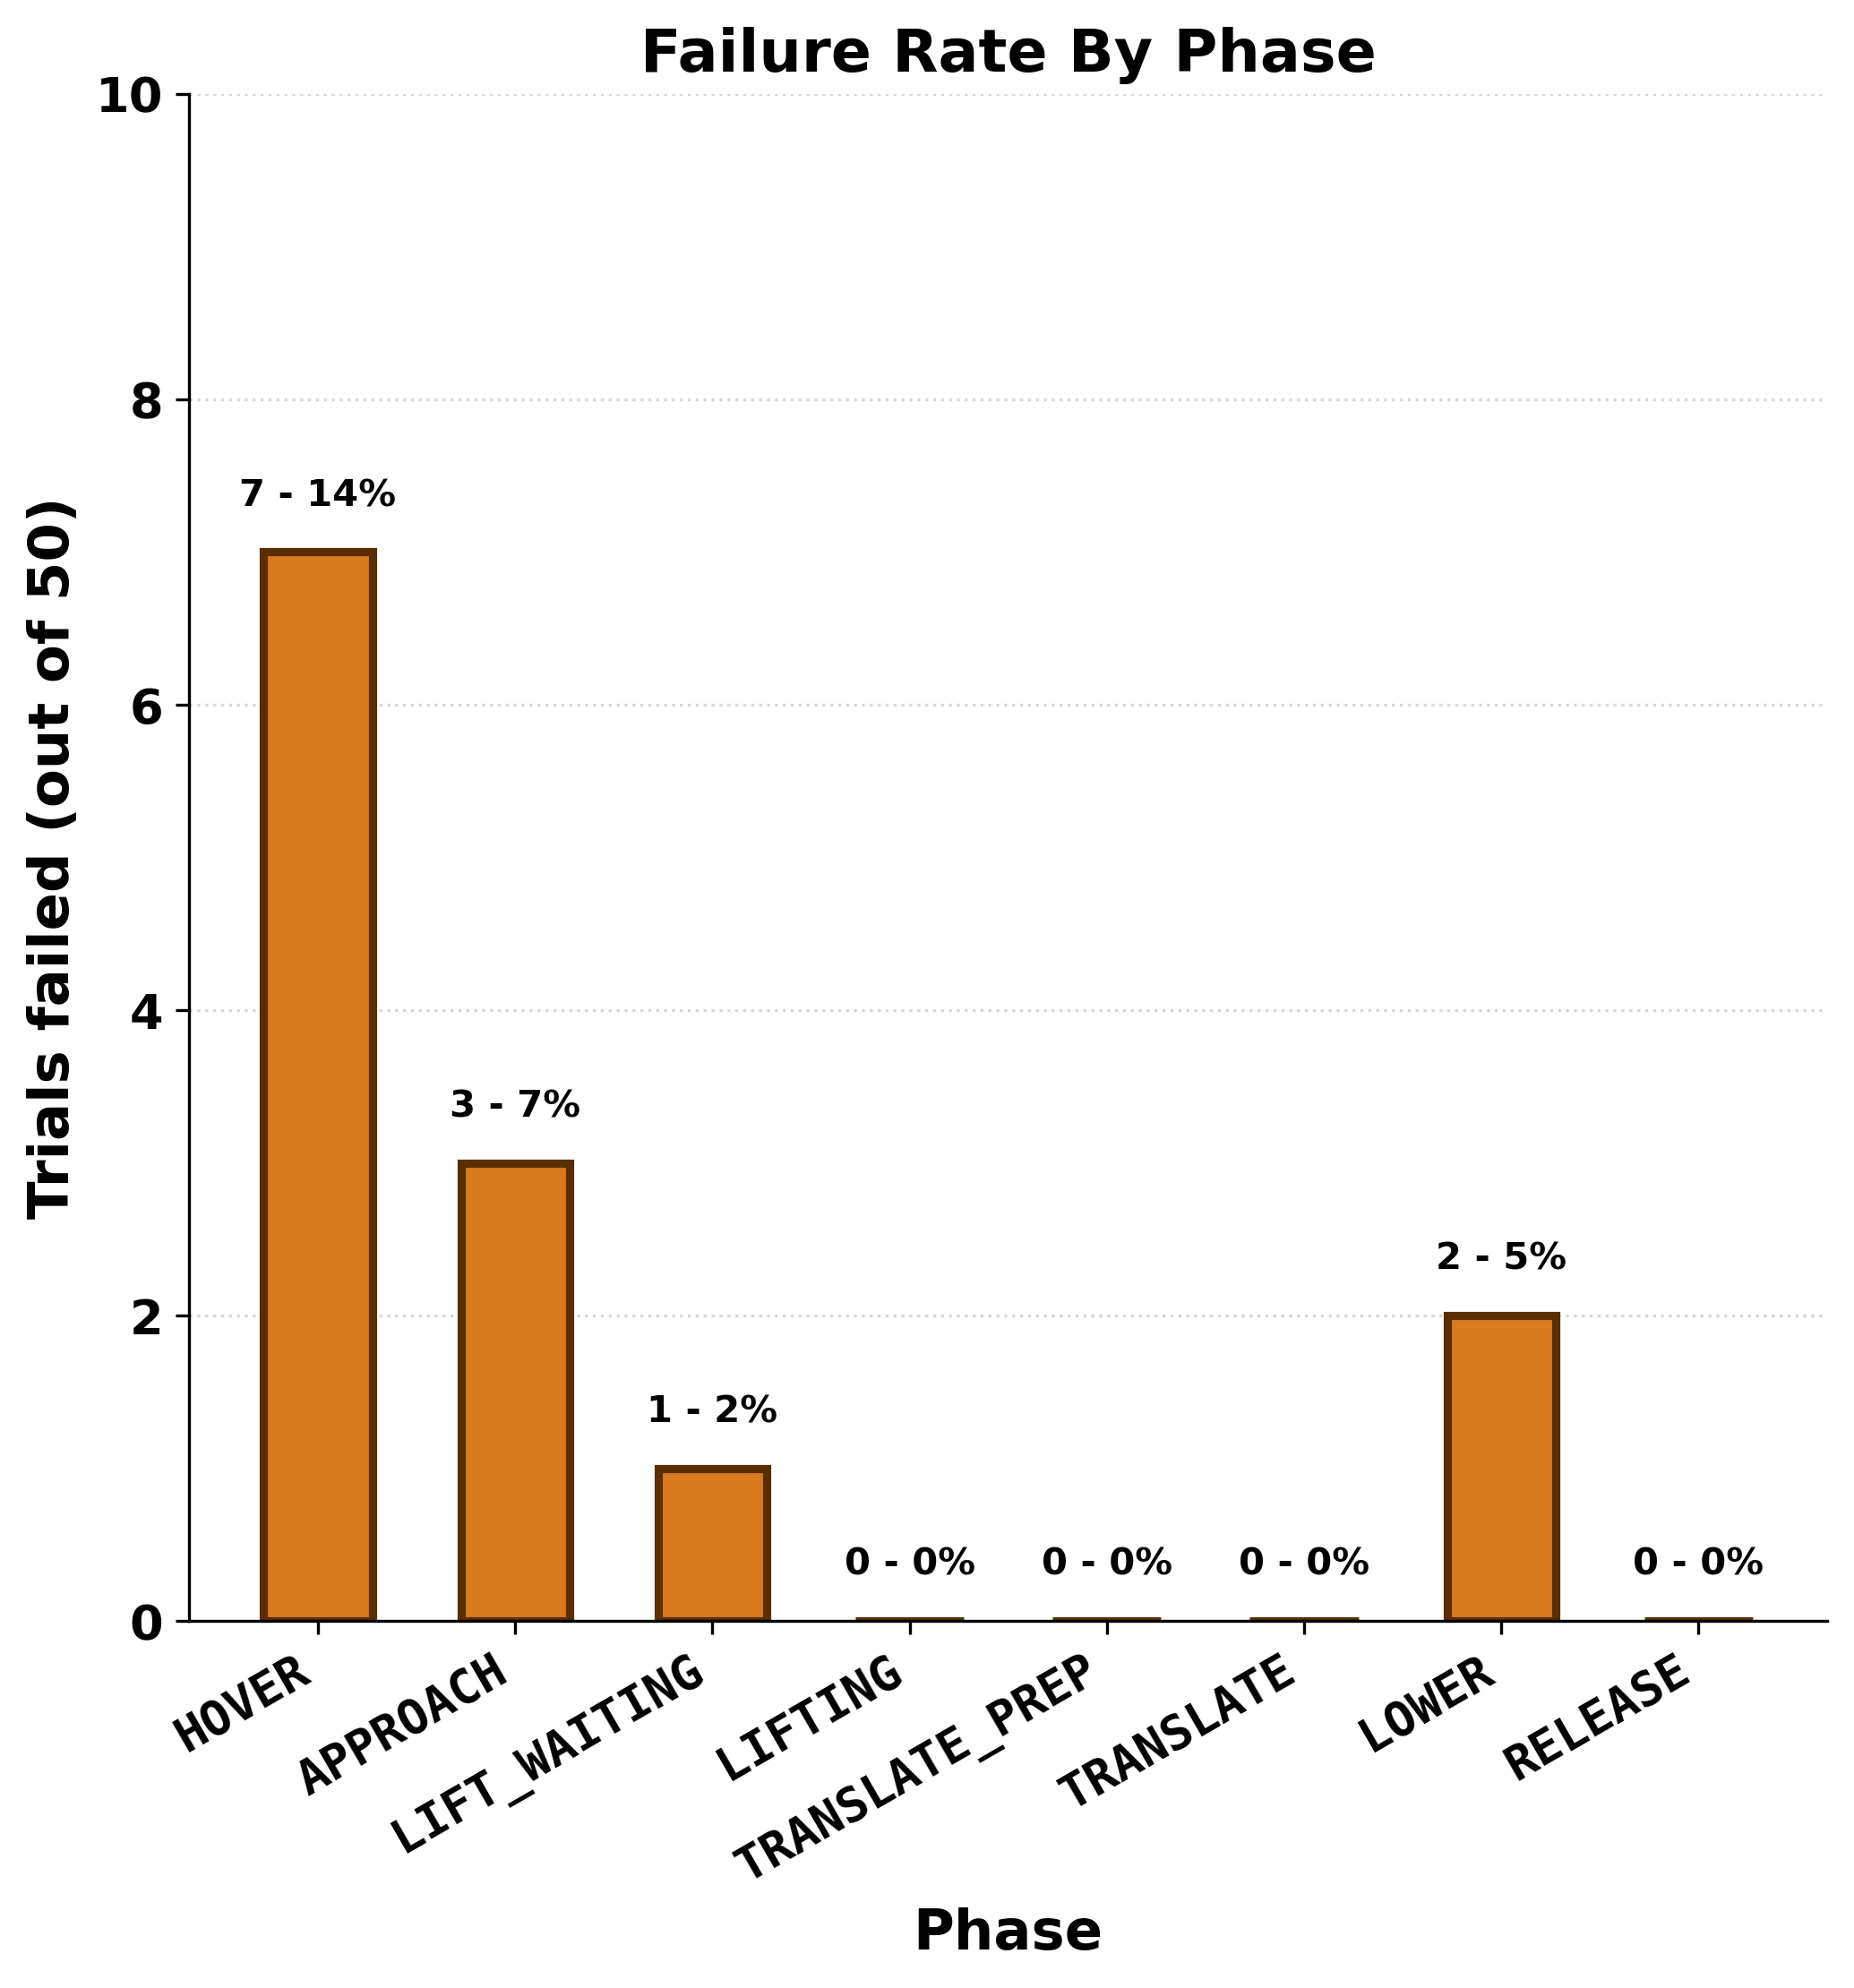
\includegraphics[width=1\linewidth]{subtex//images/failure_rate_by_phase.png}
    \caption{Failures and failure rates during 50 trials. Percentages represent failure rate relative to the total number of trials that made it to that phase.}
    \label{fig:failure rate per phase}
\end{figure}


The failure modes for each phase are described below. 
\newline

\textbf{\texttt{HOVER} (7\,/\,50, 14\%).} \texttt{HOVER} is the most failure-prone phase, with two distinct failure modes. In the more common mode, the arm converges to a position slightly offset from the actual tray marker. This is close enough that the convergence test passes, but offset enough that on APPROACH the gripper hits the tray. This failure traces directly to \texttt{POSITION\_OFFSET} (Section \ref{sec:hover}), which was the only parameter in the entire pipeline that required precise per-arm tuning very often. The second failure mode is a non-convergence where the planar error never falls below \texttt{CONVERGENCE\_THRESHOLD\_M} for three consecutive frames, and the arm stalls in HOVER indefinitely. Loosening the threshold trades one mode for the other.

\textbf{\texttt{APPROACH} (3\,/\,43, 7\%).} \texttt{APPROACH} has no closed-loop correction during descent as it just steps straight down from wherever \texttt{HOVER} ended with a descent delta. These pre-alignment problems are considered \texttt{HOVER} failures, but have the potential to be remedied by this phase. When the gripper was aligned, however, and the descent caused a misalignment, or the arm did not descend the right amount, an \texttt{APPROACH} failure was recorded. A potential future fix is to implement visual servoing during the descent rather than cutting to a fixed delta, which would help this phase as well as the previous, but requires inverse kinematics outside the motion map plane.

\textbf{\texttt{LIFT\_WAITING} (1\,/\,40, 2.5\%).} A single trial failed when one arm's nudge produced a tray-marker rise below \texttt{TAG\_RISE\_THRESHOLD\_M} $= 3$\,mm. The handshake is designed to refuse false positives, so the listening arm waited indefinitely and the system just stopped. Lowering the threshold would have caught this trial but would also raise the chance of false positive triggering due to measurement jitter. Increasing the nudge-lift magnitude would also fix this problem, but increases the risk of tilting the tray too much and causing the glass to move or spill.

\textbf{\texttt{LOWER} (2\,/\,39, 5\%).} Both \texttt{LOWER} failures were due to the same failure mode. One arm reached the end of its lowering trajectory while still seeing itself as the lower side by more than \texttt{TILT\_PAUSE\_THRESHOLD\_M} $= 5$\,mm, so the tilt-pause rule of \cref{algo:lower} held it indefinitely and the gripper never released. To fix this, more accurate lowering waypoints during data collection around the table contact height would close this gap. It was never the case that the arms released before the tray had reached the table, so a slightly higher waypoint would be beneficial.

\textbf{Phases with zero failures.} \texttt{LIFTING}, \texttt{TRANSLATE\_PREP}, \texttt{TRANSLATE}, and \texttt{RELEASE} produced no failures across all trials that reached them. The successful synchronized lift is attributable to \cref{algo:lift}'s self-throttling rule. The translate phases benefited from the TPU gripper tips, whose flexibility absorbed small marker jitter and pose mismatches that would otherwise have caused tray slippage. The hardcoded phases at the beginning and end also never failed since those were done as a simple interpolation between two points.



\subsection{Coordination Metrics}

\begin{figure} 
  \centering
  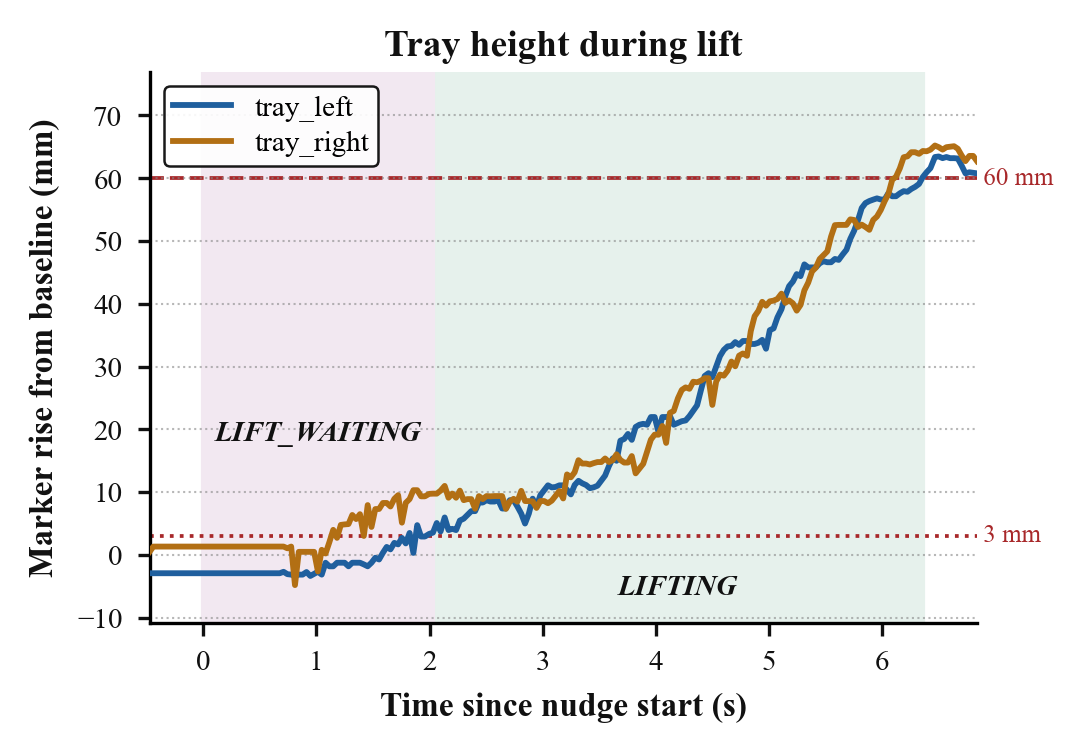
\includegraphics[width=1\columnwidth]{subtex/images/lift_height.png}
  \caption{Synchronized ascent produced by the self-throttling rule
  of \cref{algo:lift}. Each arm only commands an upward step when
  its own side is at or below the other side.}
  \label{fig:lift}
\end{figure}

\begin{figure}
\centering
  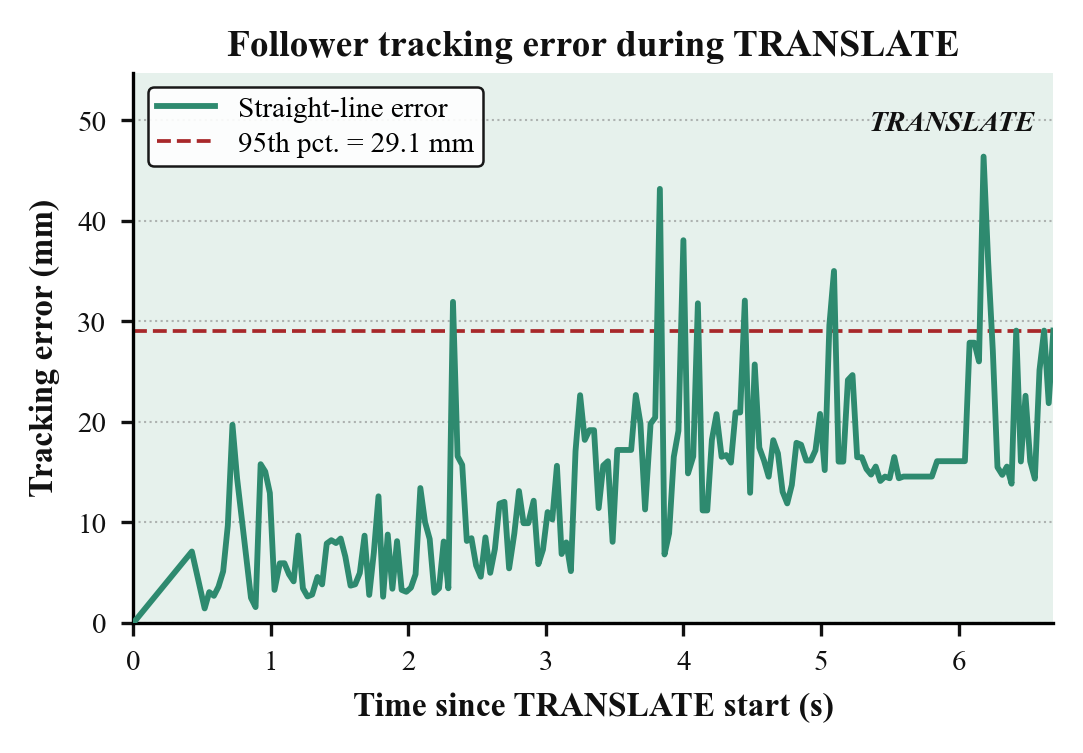
\includegraphics[width=1\columnwidth]{subtex/images/translate_follower_error_ep004.png}
  \caption{Follower tracking error during \texttt{TRANSLATE} for a
  representative trial. Defined as
  $\Vert\,\vec{x}_{\text{grip},R}(t) - (\vec{x}_{\text{grip},L}(t) +
  \vec{o})\,\Vert$. The follower starts close to the desired position, but drifts further from the goal position as the leader moves away.
  The strong EMA on the follower's
  target ($\alpha_f{=}0.1$, \cref{algo:translate}) intentionally
  trades latency for rejection of the very high measurement noise.}
  \label{fig:translate-error}
\end{figure}




% these directly should reference the graophs
A simple pass or fail does not capture how cleanly the coordination ran on a successful trial. Two quantitative signals were tracked in order to best characterize the quality of the coordination:
\begin{itemize}
  \item \textbf{Tray heights.} The maximum $|y_{\text{tray},l}-
        y_{\text{tray},r}|$, or tray-marker height disagreement, observed during \texttt{LIFTING}. This measures how well \cref{algo:lift}'s self-throttling rule keeps the tray level and is shown in \cref{fig:lift}. A desynchronized nudge-lift is evident in the graph, followed by a flat region for the right arm as it waits and watches for the left arm's lift. Once both arms transition to lifting, they form this beautiful reciprocating pattern in which each arm becomes the higher one, then waits. The maximum tray tilt during this trial is approximately one centimeter, which corresponds to a maximum tray angle of 4$^\circ$ given the 14 cm marker spacing. This is much less than the tilt required to cause movement of the glass.
  \item \textbf{Translation follow error.} Shown in \cref{fig:translate-error}, this is the 3D base-frame distance from the right grip target
        ($\vec{x}_g^\text{\,left}+\vec{o}$) to the right gripper's actual position during \texttt{TRANSLATE}, with the follower tracking the leader's gripper per Algorithm \eqref{eq:offset}. The motion during each trial is quite smooth so evidently there is very high measurement noise from one or both markers. This success is attributed to the mechanical design and material improvements of the end effector assembly, as well as the EMA during control.  
\end{itemize}


\section{Discussion and Conclusion}
\label{sec:conclusion}
We have shown that a physically coupled, contact-rich bimanual task can be executed by two independent manipulators that share
only a camera and exchange no messages. We found that the coordination problem reduces, in this setting, to a design problem: choose visual signals such that (a) both arms can measure them reliably, and (b) local rules on those signals provably produce the globally-synchronized behavior the task requires.

The four coordination algorithms of \cref{sec:coordination} fit this pattern cleanly. The nudge-lift handshake is a physical act-and-observe protocol. The tilt-aware lift and lower rules
(\eqref{eq:lift-gate} and \cref{algo:lower}) are one-line local
decisions that converge to synchronized behavior because both arms evaluate the same inequality on the same measurements. The
leader-follower translation guarantees spacial awareness of the tray using the gripper markers, avoiding the tray-bending failure mode that caused problems in the symmetric implementation.

\subsection{Limitations}
Three limitations deserve an explicit discussion.
\begin{itemize}
  \item \textbf{Shared-camera assumption.} A genuinely decentralized version of this system would need each arm to carry its own camera. The motion-map would work well once the base-frame transform is in place, but individual arm cameras would induce per-arm errors when reading all of the markers. These errors would propagate the most in the \texttt{HOVER} and \texttt{TRANSLATE} phases, in which the arms currently require the most precise measurements. Quantifying the tolerance of our algorithms to such errors is left to future work. Additionally, the current positioning of the fiducial markers would not be visible to the arms in most of their orientations, as they are designed to face a nearby camera. Resolving this would likely require a different perception solution entirely, as marker occlusion would become a significant failure mode.
  \item \textbf{Workspace coverage.} The polynomial motion map is only valid inside the recorded sweep, at the swept height. Queries outside the bounds are rejected rather than extrapolated, which, on some occasions, means an aggressively placed tray can leave an arm stalled in \texttt{HOVER}. A better solution would fix the problems with the current motion map's extrapolation or implement precise inverse kinematics that are situation-aware and know which DoF can be sacrificed in varying circumstances.
  \item \textbf{Lack of generalizability.} The \texttt{HOVER} algorithm was intended to be able to track the tray anywhere in the reachable area. In practice, this is not the case. It reliably locates the tray in a small radius around the starting point, but it usually fails to pick up the tray when it is placed in far away, but physically reachable locations. We concluded that this is a combination of motion map error in the extremities of the region and lack of precise control over servo timing. Expanding on the second idea, it frequently was the case that the arms would swoop towards the tray in a low arc that intersects and pushes the tray before the arms arrive. A preliminary idea to remedy this is delaying the joints that cause the arm to lower for a short period, while the joints responsible for raising realize their positions. The effect of this would ideally be an arm that moves in from above instead of from below. This was never implemented because of a large array of error accumulation and latency concerns.

  On a similar note, the final position of the tray is also not generalizable. We can re-record the waypoints used throughout the script to change where the tray will arrive, but this would likely require re-tuning a host of parameters and is clunky. A better and more field-applicable solution would allow the user to choose a destination position in space (potentially as arguments on the file call), and the tray would arrive there.
\end{itemize}

\subsection{Future Work}
The most interesting extension is to preserve the no-communication constraint while moving each arm to its own independent perception stack with a separate camera, a separate processor, and no AprilTag IDs. This would require agreeing on object identity through vision alone (potentially by color, shape, or ML embeddings), replacing the marker-based pose estimates with an ML detector, and quantifying the resulting drop in coordination quality. I would expect an extreme drop in quality on the current hardware. 

A second direction is to push the motion map toward 3D to remove the hover-plane assumption, which would let the same coordination primitives drive non-planar tasks such as orienting or tilting the tray intentionally. This would broaden the capabilities of the system and improve the generalizability, while staying true to the idea of a motion map. We actually considered utilizing a 3D motion map, but our 2D map demanded 2400 hand-collected data points (of which we were only able to collect 70\%) and a 3D map would require at least 5-10 times that to be useful. 

A final interesting direction would be to implement the algorithms we have presented here on more capable hardware. We expect that high-DoF production-quality robotic arms would have no problem completing this task, but many of the algorithmic design alterations are a direct result of this hardware. Changing that variable might produce unpredictable results.

\subsection{Conclusion}
Coordination without communication is not only possible but
practical for contact-rich bimanual tasks, provided the scene is
instrumented so that the signals two agents would otherwise
exchange are instead visible in a shared image. The system presented here is a concrete demonstration: small, understandable algorithms, a simple polynomial motion map, and a shared finite-state protocol are enough to lift and translate a tray with a water glass, reliably, on two arms that never speak to each other.


\section{Author Contributions}
\label{sec: author contributions}

\begin{table} [H]
    \centering
    \begin{tabular}{|c|c|}\hline
         Section& Author\\\hline
         Abstract & Both\\\hline
         Introduction& Jackson\\\hline
         Related Work& Both\\\hline
         System Overview& David\\\hline
         Perception and Base-Frame Calibration& David\\\hline
         The Motion Map& Jackson\\\hline
         Emergent Coordination via Shared Vision& Jackson\\\hline
         Experimental Evaluation& David\\\hline
 Discussion \& Conclusion&Jackson\\ \hline
    \end{tabular}
    \caption{Paper Contributions}
    \label{tab:paper contributions}
\end{table}


\begin{table} [H]
    \centering
    \begin{tabular}{|c|c|}\hline
         Project Task& Engineer\\\hline
         Hardware/CAD Design \& Modifications& David\\\hline
         Fabrication \& Assembly& Both\\\hline
         Camera \& Workspace Setup& David\\\hline
         Perception Pipeline& David\\\hline
         Motion Map \& Data Collection& Jackson\\\hline
         Coordination Algorithms& Jackson\\\hline
         System Integration/Testing& Both\\ \hline
    \end{tabular}
    \caption{Project Task Contributions}
    \label{tab:project task contributions table}
\end{table}



\bibliographystyle{IEEEtran}
\bibliography{IEEEabrv,references.bib}



% that's all folks
\end{document}

   
  
 
